%========================================
% PREAMBOLO
%========================================

% === Impostazione del documento ==========================
\documentclass[a4paper,12pt,twoside,english,hidelinks]{report}
\pagenumbering{arabic}
\usepackage{setspace}
\onehalfspace

% === Regolazione dei margini =============================
\usepackage{geometry}
\geometry{a4paper, top=2.5cm, bottom=3cm, left=3.0cm, right=3.0cm, heightrounded, bindingoffset=5mm}

\addtolength{\oddsidemargin}{30pt}
\addtolength{\evensidemargin}{-30pt}
\usepackage{fancyhdr}
\usepackage{multirow}
\usepackage{multicol}
\usepackage[section]{placeins}

% === Impostazione dei font ===============================
\usepackage[T1]{fontenc}
\usepackage[utf8]{inputenc}
\usepackage[english]{babel}
\usepackage{ae}
\usepackage{relsize}
\usepackage{csquotes}
\usepackage{quoting} 
\usepackage{amsmath}
\usepackage{amsfonts}
\usepackage{amssymb}
\usepackage{pifont}
\usepackage{mathdots}
\usepackage{mathtools}
\usepackage[colorlinks=true]{hyperref}
\hypersetup{
	bookmarksnumbered=true,
	linkcolor=black,
	citecolor=black,
	pagecolor=black,
	urlcolor=black,
}
\usepackage{verbatim}
\usepackage{alltt,footnote}
\DeclareMathOperator{\sgn}{sgn}
\DeclarePairedDelimiter{\abs}{\lvert}{\rvert}
\DeclarePairedDelimiter{\norma}{\lVert}{\rVert}
\usepackage{enumitem}
\usepackage{textcomp}
\usepackage{syntonly}
	\usepackage{microtype}
\usepackage{indentfirst}

% === Integrazione delle figure ===========================
\usepackage{graphicx}
\graphicspath{{./PICTURES/}}
\renewcommand{\figurename}{Fig.}
\usepackage{subfig}

% === Per gli algoritmi ===================================
\usepackage{algorithmicx}
\usepackage[ruled]{algorithm}
\usepackage{algpseudocode}
\usepackage{xcolor}
\usepackage{listings}

% === Per le tabelle ======================================
\usepackage{tabularx}
\usepackage{array}
\usepackage{color}
\usepackage{colortbl}
\usepackage{longtable}
\usepackage{pgfplotstable}
\usepackage{makecell}
\usepackage{booktabs}

%==Per le figure latex======================================
%Package e librerie per TikZ e PGF, le librerie non sono tutte necessarie a questo documento LATEX.
\usepackage{tikz,fp,ifthen,fullpage,pgfmath,xparse,tikz-dimline}
\usetikzlibrary{decorations,backgrounds,fit,calc,through}
\usetikzlibrary{arrows,shadows,shapes}
\usetikzlibrary{fadings,patterns,mindmap}
\usepackage{pgfplots}
\pgfplotsset{compat=1.13}


%==Per APDL e linguaggi======================================          
\usepackage{listings}
\usepackage{xcolor}
% === APDL STYLE LANGUAGE ==================================
%colori per il linguaggio
\definecolor{darkpastelpurple}{rgb}{0.59,0.44,0.84}
\definecolor{halfgray}{gray}{0.55}
\definecolor{arylideyellow}{rgb}{0.91,0.84,0.42}
\definecolor{cadmiumgreen}{rgb}{0.0,0.42,0.24}
\definecolor{ceruleanblue}{rgb}{0.16,0.32,0.75}
\definecolor{cinnamon}{rgb}{0.82,0.41,0.12}
\definecolor{darkslateblue}{rgb}{0.28,0.24,0.55}
\lstdefinelanguage{apdl-modified}
{
	alsoletter=/*\%,
	morekeywords={/clear,/filnam,/title,/unit,/inquire,/rep,/ang,/eshape,/replot,/view,/exit,/replo,/plopts,/triad,/efacet,/rgb,/show,/gile,/eof,/solve,/output,/out,/device
	},
	morekeywords={*afun,*dim,*vget,*do,*enddo,*cfopen,*vwrite,*cfclos,*set,
		*get,*use,*abbr,*msg,*if,*else,*endif,*abset,*abcheck,*abfini},
	morekeywords={start,new,finish,si,antype,static,set,deg,num,max,min,dim,
		count,line,llist,lplot,pngr,fast,leng,arotat,allsel,lsel,s,a,r,u ,
		none,acel,pstres,dl,mxpand,modopt,lumpm,d,save,eplot,modal,plnsol,
		sum,eqv,loc,eq,then,k,n,e,et,mp,ex,nuxy,dens,latt,lmesh,lesise,
		sectype,secoffset,secdata,keyopt,mshkey,ksel,nesl,lsel,kp,
		node,line,sect,mshape,amesh,aesize,secnum,type,real,
		mat,nslk,nsel,cyl4,wpcsys,csys,wpoffs,wprota,cerig,
		secjoint,joint,revo,esel,cm,elem,ui,x,y,z,
		lesize,solve,pldisp,sequ,l,mode,freq,coriolis,qrdamp,
		wpstyle,fill,secd,nsll,clocal,outpr,elform,elprep,nplot,psolve,
		secp,ncomp,cdsys,rect,csolid,etyp},
	otherkeywords={/angle},
	keywords=[2]{beam188,beam189,shell181,mpc184,combin14,mass21},
	keywords=[3]{/prep7,/solu,/post1,/post26},
	keywords=[5]{ARRAY,TABLE},
	keywords=[4]{
		',
		-,
		",
		\%,
		(,
		),
		,,
		.,
		:,
		;,
		?,
		^,
		−,
		+,
		<,
		=,
		>,
		e,
	},
	%define string
	morestring=[b]\%,
	morestring=[b]',%
	morestring=[b]",%
	morestring=[s]{r'}{'},% `raw' strings
	morestring=[s]{r"}{"},% `raw' strings
	morestring=[s][\color{red}\bfseries]{\%}{\%},% `raw' strings
	sensitive=false,% keywords are not case-sensitive
	%define comment
	morecomment=[l]{!},
	morecomment=[l]{/COM},
}
\lstset{
	%Frame style
	frame=single,
	rulecolor=\color{black},
	%number style
	numbers=left,
	numberstyle=\tiny\color{halfgray},
	%space and special character
	showspaces=false,
	showstringspaces=false,
	showstringspaces=false,
	breaklines=true,
	%input path
	%inputpath={{/}},
	extendedchars=true,
	literate=
	{á}{{\'a}}1 {é}{{\'e}}1 {í}{{\'i}}1 {ó}{{\'o}}1 {ú}{{\'u}}1
	{Á}{{\'A}}1 {É}{{\'E}}1 {Í}{{\'I}}1 {Ó}{{\'O}}1 {Ú}{{\'U}}1
	{à}{{\`a}}1 {è}{{\`e}}1 {ì}{{\`i}}1 {ò}{{\`o}}1 {ù}{{\`u}}1
	{À}{{\`A}}1 {È}{{\'E}}1 {Ì}{{\`I}}1 {Ò}{{\`O}}1 {Ù}{{\`U}}1
	{ä}{{\"a}}1 {ë}{{\"e}}1 {ï}{{\"i}}1 {ö}{{\"o}}1 {ü}{{\"u}}1
	{Ä}{{\"A}}1 {Ë}{{\"E}}1 {Ï}{{\"I}}1 {Ö}{{\"O}}1 {Ü}{{\"U}}1
	{â}{{\^a}}1 {ê}{{\^e}}1 {î}{{\^i}}1 {ô}{{\^o}}1 {û}{{\^u}}1
	{Â}{{\^A}}1 {Ê}{{\^E}}1 {Î}{{\^I}}1 {Ô}{{\^O}}1 {Û}{{\^U}}1
	{œ}{{\oe}}1 {Œ}{{\OE}}1 {æ}{{\ae}}1 {Æ}{{\AE}}1 {ß}{{\ss}}1
	{ç}{{\c c}}1 {Ç}{{\c C}}1 {ø}{{\o}}1 {å}{{\r a}}1 {Å}{{\r A}}1
	{€}{{\EUR}}1 {£}{{\pounds}}1 {θ}{{$\theta$}}1 {Φ}{{$\Phi$}}1,
	% defie style
	basicstyle=\scriptsize\ttfamily,
	% style of keyword
	% keyword
	keywordstyle=\color{ceruleanblue}\bfseries\ttfamily,
	%type elements
	keywordstyle=[2]\color{darkslateblue},
	% section
	keywordstyle=[3]\color{cinnamon},
	keywordstyle=[4]\color{black},
	keywordstyle=[5]\color{arylideyellow},
	% style of comments
	commentstyle=\color{cadmiumgreen}\ttfamily,
	% style of string
	stringstyle=\color{darkpastelpurple}\ttfamily,
} 




\usepackage{appendix}

%========================================
% TESTO REPORT
%========================================

\begin{document}
	
	% === Frontespizio ====================================
	\pagestyle{empty}
	%%%%%%%%%%%%%%%%%%%%%%%%%%%%%%%%%%%%%%%%%%%%%%%%%%%%%%%%%%%
% Frontespizio
%%%%%%%%%%%%%%%%%%%%%%%%%%%%%%%%%%%%%%%%%%%%%%%%%%%%%%%%%%%
\begin{titlepage}
 \begin{center}
 
\includegraphics[width=3.5cm]{unitn.jpg}\\
 \vspace{1em}
 {\Large \textsc{Università degli studi di Trento}}\\
 \vspace{1em}
 {\Large \textsc{Dipartimento di Ingegneria Industriale}}\\
 \vspace{4em}
 {\normalsize Relazione}\\
 \vspace{1em}
 {\Large \textsc{Mechanical Vibrations}}\\
 \vspace{4em}
 {\LARGE\textbf{
 	System identification of a 3 DOF system
 }}\\
 \end{center}

\vskip 2.0cm
 \begin{center}
 \begin{tabular}{c c c c c c c c}
 Relatore & & & & & & & Candidato \\[0.2cm]
 \large{Prof. Daniele Bortoluzzi} & & & & & & & \large{Francesco Aregntieri}\\[0.4cm]
 Correlatore & & & & & & & ID: 183892\\[0.2cm]
 \large{Dott. Egidio Labbate}& & & & & & &\\
 \end{tabular}
 \end{center}

\vskip 1.5cm
\begin{center}
{\normalsize Anno Accademico 2015/2016}
\end{center}
\end{titlepage}

\clearpage{\pagestyle{empty}\cleardoublepage}

	
	%%%%%%%%%%%%%%%%%%%%%%%%%%%%%%%%%%%%%%%%%%%%%%%%%%%%%%%%%%%%%%%%%
	
	\pagestyle{empty}
	
	\begin{abstract}
		This document is aimed to be a report of the work performed during the master course of \emph{Modeling and Design with Finite Elements}, for the part about the course's project, developed in team with ANSYS Mechanical APDL Software. \\ 
		
		\noindent
		The purpose is to present a consistent finite-element formulation, developed to predict the free vibration characteristics of two different helicopters tailboom structures. \\ Both airframes considered for our analysis are taken from real-world widespread helicopters types; the first model regards the tail of a \textbf{Lama SA-315b} which is an old type of reticular steel structure, quite easy to design and manufacture, while the second model represents a modern semi-monocoque tail design that consists in an ensemble of an aluminium skin layer connected with other structural elements and commonly adopted in modern rotor-craft's airframes like the one of the \textbf{Eurocopter AS-350 ecureuil}. \\
		
		\noindent
		The work has been organized in a sequence of \underline{steps of increasing complexity and accuracy}. \\ Initially the problem has been approached by independent investigations of the free vibrational behaviour of the two different airframes (\emph{uncoupled tailrotor-fuselage dynamic model}). Thus, results are obtained for the naked structures only. Then, the tailboom's models have been improved taking into account also the presence of additional subsystems normally fixed on helicopter's tail and the system's natural frequencies have been re-calculated. Furthermore, some theoretical hints on how to take into account the \emph{tailrotor-fuselage dynamic coupling}, which considers also the interaction of the effects related to the the tail-rotor rotation, have been presented in the chapter 4. This last step is quite ambitious, the topic is wide and complex, however it should be considered to develop a model which is accurate enough to study the real system's vibrational behaviour. \\
		
		\noindent
		  The last part, instead, is aimed to explore the Ansys' Rotor-dynamic capabilities and tools which are only recently implemented in the software. A great deal of efforts have been done to understand the physical phenomena and try to implement a simple model from the rotor-dynamics point of view. However, this can be done only under important simplifying assumptions. For our purposes, this part is only limited to study the rotor's vibrational behaviour which turns to be velocity dependent (varies with tail rotor speed). \\ 
		
		
		%  In fact, \underline{a simplified elastically-suspended rotor} has been considered and it has %been modelled as a rigid disk (actually as an annular ring of material) which rotates around an %elastic beam's shaft fixed on the tail by two elastic bearings. \\
		
		
	\end{abstract}
	
	\clearpage
	\newpage %PAGINA VUOTA
	\null
	\pagestyle{empty}
	\newpage
	
	%%%%%%%%%%%%%%%%%%%%%%%%%%%%%%%%%%%%%%%%%%%%%%%%%%%%%%%%%%%%%%%



	% === Indice ==========================================
	\tableofcontents
	\pagestyle{headings}
	\setcounter{page}{3}


	% === Capitoli Report ===================================
	\pagestyle{plain}
	\chapter*{INTRODUCTION}
\addcontentsline{toc}{chapter}{INTRODUCTION}
\addcontentsline{toc}{section}{General overview and motivations}
\noindent
\emph{Helicopter's vibrations} is a long-standing problem. Since the earliest days of rotor-craft development, oscillatory motion of the non-rotating portion of the airframe has been a matter of serious concern, from several viewpoints. \\ In fact, one of the reasons is that typically \emph{oscillatory motions} mean \emph{oscillatory strains} and oscillatory strains often involve \emph{fatigue of structural components} which affect the service life, increase the maintenance costs, reduce the availability of the machine and the safety of the flight itself. \\
Similarly, vibrations constitute a problem for equipments of all kinds; they make instruments hard to read, sight hard to aim and the add to fatigue of pilots, crew and passengers. \\

\noindent For these and many other reasons, vibration is an unwanted phenomenon in rotor-craft's design and operations and must be seriously faced by engineers since the beginning. \\
Unfortunately, helicopters are really complex machines with many rotating components and so they are intrinsically subject to vibrations which must be reduced or damped. \\

\medskip
\begin{figure}[h]
	\begin{center}
		\centering  		 		
		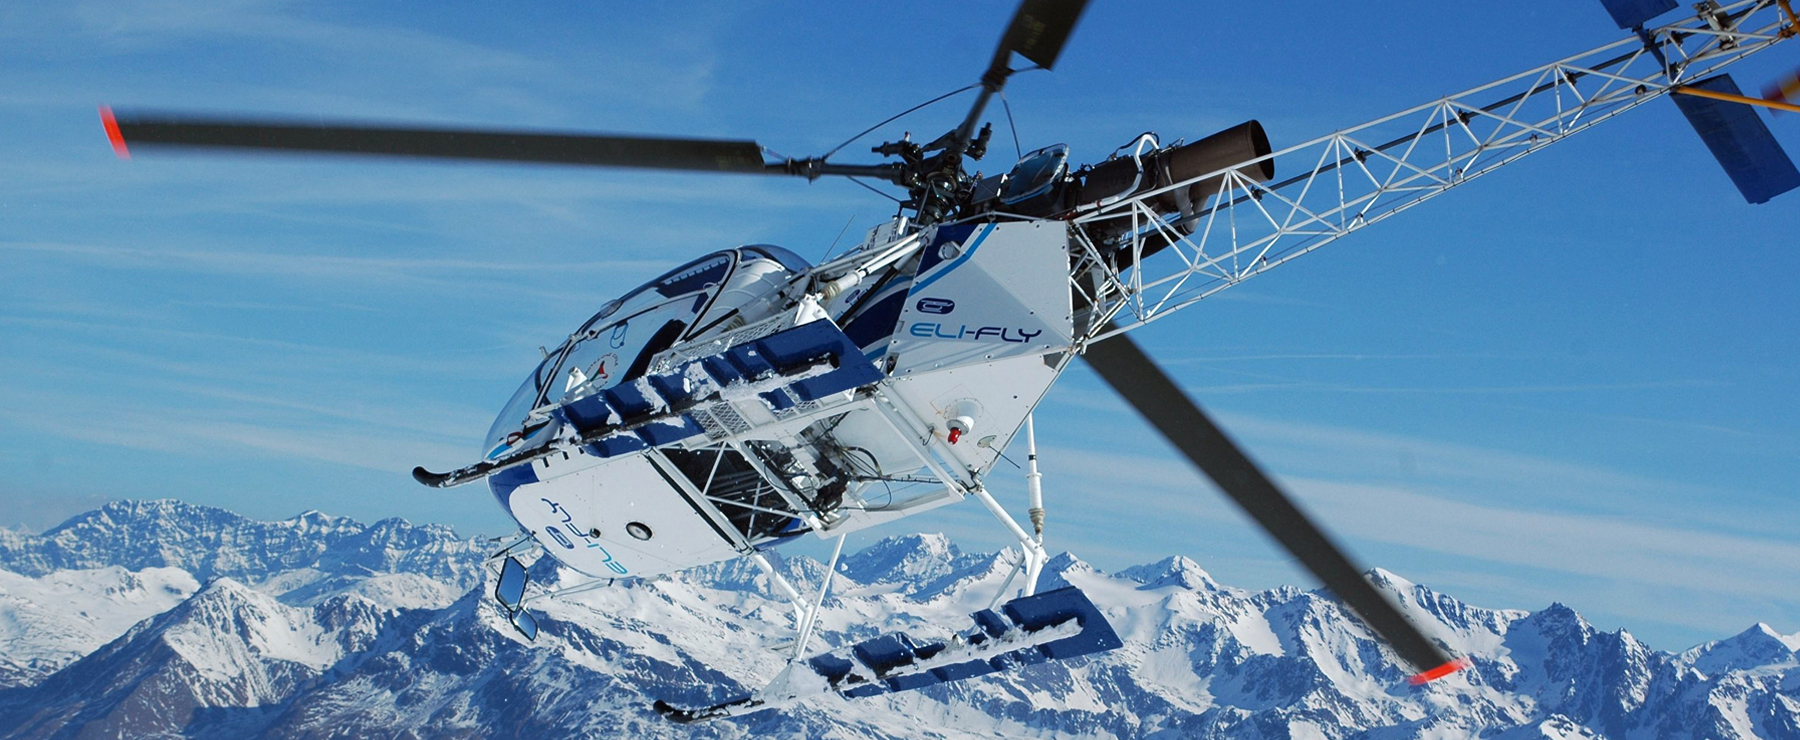
\includegraphics[width=1\linewidth]{PICTURES/Introduction/PNG/Elicottero_montagne.jpg}
	\end{center}
	\caption {A turbine helicopter during an in-flight manoeuvre}
\end{figure}
\vspace{0.5cm}

\noindent
There are many \underline{sources of vibration excitation} in a helicopter: for example,
\begin{itemize}
	\item engine and gearbox vibratory forces;
	\item main and tail-rotor excitations;
	\item rotor-mass imbalance;
	\item inertial and centrifugal accelerations due to manoeuvres during the flight. 
\end{itemize}

\bigskip
\noindent
Although the tail rotor causes a lesser effect then the main rotor on the overall vibration of the helicopter, its effects cannot be neglected especially because \emph{airframe vibrations are also typically amplified cause of the lightweight and flexible fuselage design}. \\
The primary causes of rotating machinery vibration are unbalances, misalignments, looseness and the excitation of structural resonances by rotating shaft running frequencies and their harmonics. Other sources of vibration can be bearing defects, insufficient lubrication and dirt entrapment between moving or rotating surfaces. \\
Excessive vibration of tail rotor can cause the tail section of helicopters to be physically ripped from the main structural assembly, and result in catastrophe. Severe imbalance in the rotating parts also can lead to instabilities during flight. \\

\noindent
Unfortunately, \underline{the complete helicopter vibration problem is virtually impossible to predict} \underline{accurately}, as yet, because of its structural, as well as aerodynamic, complexity. \\
To make the helicopter vibration problem more tractable, \emph{simplifying assumptions} must be made, especially for the rotor-dynamics analysis. Typically, the rotor system and the fuselage are analyzed separately and then attempts are made to account for rotor-fuselage coupling.
However, this procedure is questionable because it does not account for rotor-fuselage coupling. 
Even introducing an equivalent rotor mass, although it gives a somewhat better approximation, still does not adequately represent the coupled rotor-fuselage system. Thus, there appears to be no viable alternative to carrying out a coupled rotor-fuselage analysis when one is investigating fuselage response to rotor excitation. \\

\noindent
In the past, the vibration had not been considered in design phase of a helicopter, but nowadays, in order to minimize the costs and increase the comfort on-board, the vibration is being taken into account at design
stage. \\ With this aim, \emph{\underline{there is a need to evaluate the vibration primarily obtaining a model of the} \underline{structure as accurate as possible} including all the secondary structures and subsystems in the model as well as considering the coupling between the fuselage and the rotor}. \\ This is the way we intended to approach the problem. \\


\clearpage
\subsection*{Project's goals}
\addcontentsline{toc}{section}{Project's goals}

\noindent
In order to develop an improved understanding of the tailboom and rotor vibration characteristics of a helicopter, this research project was undertaken with the following main objectives : 
\begin{itemize}
	
	\item Present the problem and its importance that has recently gained in the design and manufacturing operations of the rotor-craft companies; 
	
	\item analyze the free helicopters tailboom's vibrations developing accurate Finite Element Models of the two simplified types of tailboom structures;
	
	\item improve the models accuracy taking into account also the presence of additional subsystems
	normally fixed on helicopter's tail but neglecting, at this step, the tailrotor movement (\emph{uncoupled tailrotor-fuselage dynamic models});
	
	\item improve the understanding of the techniques and phenomena regarding the \emph{tailrotor-fuselage dynamic coupling} which considers also the interaction and the effects related to the the tail-rotor rotation presenting 3 possible ways to approach the problem;
	
	\item explore the recently implemented Ansys Rotor-dynamic capabilities and	tools building a simplified rotor model to study the rotor's vibrational behaviour which results to vary with tail rotor speed.
\end{itemize}

\bigskip
	\chapter{Theoretical concepts}


\section*{Common type of aircraft's structures}
\noindent
The structures of aircrafts have significantly changed during time and advances in materials and processes used to construct the fuselage have led to their evolution from simple wood truss structures to the sleek composite and aerodynamic flying machines of today. \\
Despite the wide variety of different shapes and geometries existing, three common basic types of structures can be highlighted at the base of aircraft's design: 
\begin{itemize}
	\item TRUSS TYPE (or tubular);
	\item MONOCOQUE / SEMI-MONOCOQUE (or stress-skin);
	\item BONDED (or composite construction).
\end{itemize}  


\noindent A brief general description of the main features of these kinds of structures is now outlined for completeness.
\smallskip
\noindent 
\subsubsection*{TRUSS TYPE (or tubular)}
\addcontentsline{toc}{section}{Truss structures}
\noindent This type of construction is typical of the early generation of airplanes and it is still in use in many lightweight aicrafts and helicopters. It is quite simple and it consists typically in \emph{welded steel tube trusses} which form a rigid frame in such a manner that all members
of the truss can carry both tension and compression loads. \\ 

\smallskip
\noindent 
\emph{Advantages}: 
\begin{itemize}
	\item High strenght to weight ratio;
	\item Simple; can be repaired at field level unless need for a jig for alignment process.
\end{itemize}


\smallskip
\noindent 
\emph{Disadvantages}: \begin{itemize}
	\item High costs of manufacturing;
	\item Difficult to hold dimensions to a close tolerance.
\end{itemize}

\smallskip
\noindent 
Normally it consists in 3 or 4 \underline{longerons} that run the entire structure's length; they took most of the compressive and tensile loads and resists to the flexural deformation. \\
Longeron are kept apart by \underline{cross members} (ideally subject only in tension / compression) which can be arranged in different configurations eg. 'N', 'X' oe 'W' to cope with the side ways loads (e.g. tail rotor thrust in helicopters). \\
\underline{Diagonal members} (or cross bracing) took the internal space and complete the structure. \\
In some aircraft, principally the light, single engine
models, truss fuselage frames may be constructed of
aluminum alloy and may be riveted or bolted into one piece,
with cross-bracing achieved by using solid rods or tubes. \\

\noindent


\smallskip
\begin{figure}[h!]
	\begin{center}
		\centering  		 		
		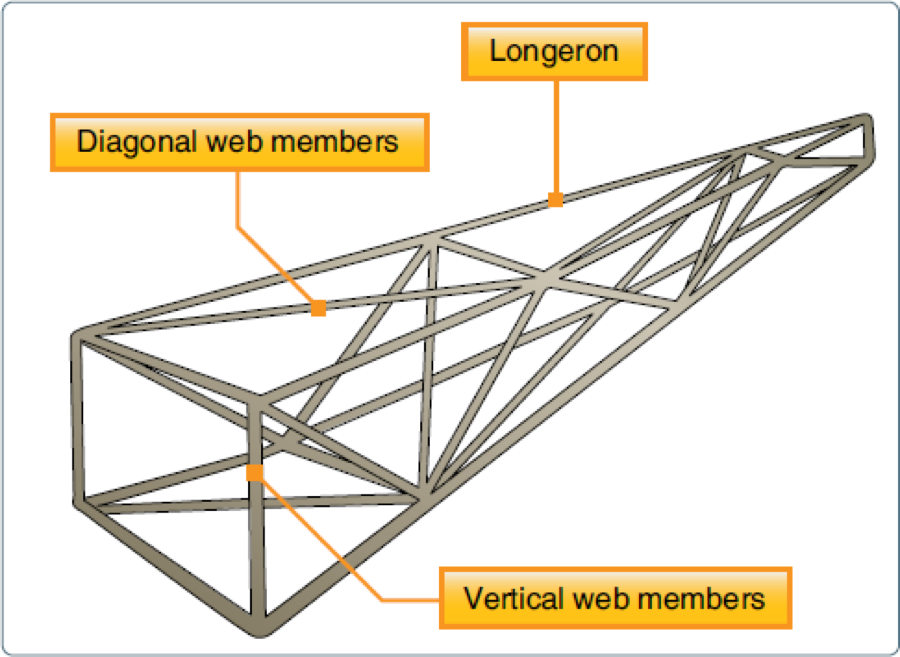
\includegraphics[width=0.7\linewidth]{PICTURES/1_Theory/PNG/truss_members.png}
	\end{center}
	\caption {Example of a Warren truss structure}
\end{figure}
%\vspace{0.5cm}



\clearpage
\noindent 
\subsubsection*{SEMI-MONOCOQUE CONSTRUCTION}
\addcontentsline{toc}{section}{Semi-monocoque construction}
\noindent This is the preferred method of constructing aluminium fuselages and can be either MONOCOQUE or SEMI-MONOCOQUE depending on the role of the outer skin. In the first case the exterior surface of the fuselage is also a primary structure so it contributes to resist external loads while in the second case it is just a coverage and helps only to resist to torsions. \\
The biggest problem involved in monocoque constructions is maintaining enough strength while keeping the weight within allowable limits. This problem is typically overcome using semi-monocoque constructions. \\
These kinds of structures consist of a series of \underline{vertical frames} in the shape of the fuselage's cross sections held in position on a rigid fixture, or jig and joined together with \underline{longerons} (typically made of aluminum alloys) which extend across several frame members and help the skin to support primary bending loads. Also lightweight longitudinal elements called \underline{stringers} can be used to further reinforcement which are typically more numerous and lighter in weight than the longerons. All these elements are in turn covered with a skin of sheet aluminium, attached by riveting. 
Most modern aircraft are considered to be of semi-monocoque type construction. \\

\smallskip
\begin{figure}[h!]
	\begin{center}
		\centering  		 		
		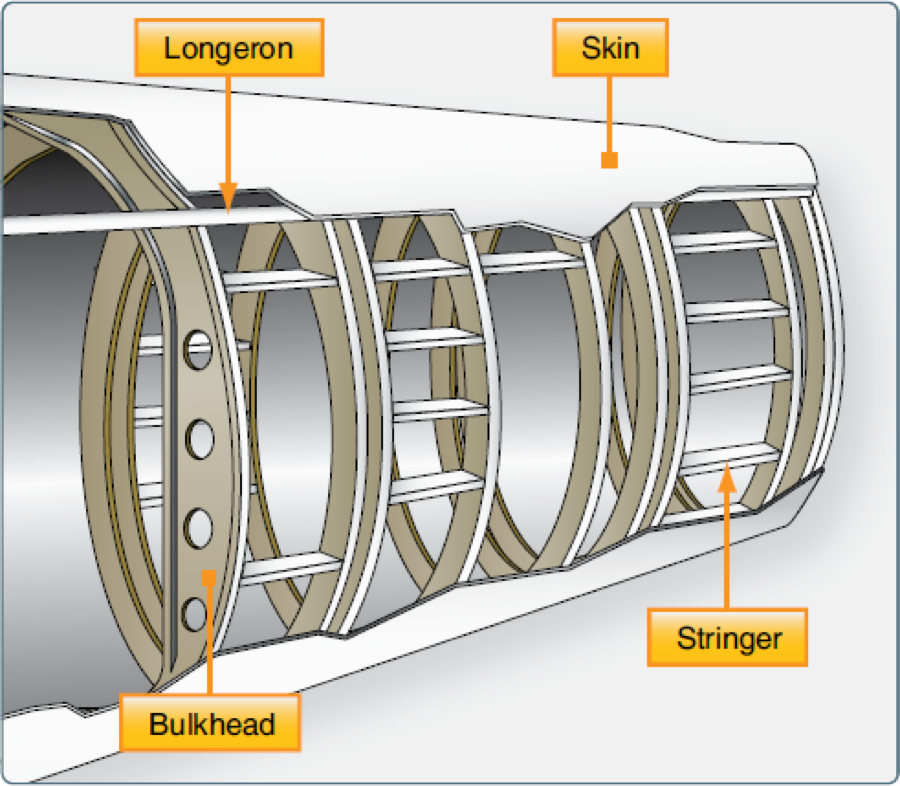
\includegraphics[width=0.7\linewidth]{PICTURES/1_Theory/PNG/semi-monocoque.png}
	\end{center}
	\caption {The most common airframe construction (semi-monocoque).}
\end{figure}
%\vspace{0.5cm}

\noindent 
The semimonocoque fuselage is constructed primarily of alloys of aluminum and magnesium, although steel and titanium are sometimes found in areas of high temperatures. \\ The fuselage skin thickness can vary with the
load carried and the stresses sustained at a particular location. \\

\smallskip
\noindent 
\emph{Advantages}: \begin{itemize}
	\item High strenght to weight ratio (higher than the truss constructions of the same size);
	\item Spreading loads among different structures and
	the skin means no single piece is failure critical;
	\item Easy to manufacture and faster;
	\item More precision in terms of fitting tolerances.
\end{itemize}

\bigskip
\noindent
 \subsubsection*{BONDED CONSTRUCTION}
 
\noindent The third type of construction involves structure whose parts are joined together by chemical methods rather than mechanical.\\ Fibreglass, honeycomb and other composite materials are used in these structures by the use of adhesives, glues, heat and pressure. \\

\smallskip
\noindent
\emph{Advantage}:
 \begin{itemize}
	\item High strenght to weight ratios, reduced construction cost by eliminating riveting and welding.
\end{itemize}




	\chapter{LAMA SA-315b (truss structure)}

\section*{Introduction}
\addcontentsline{toc}{section}{Introduction}
\noindent
 The Aérospatiale Alouette II (Lama) is a French light helicopter originally manufactured by Sud Aviation that holds the distinction of being the first production helicopter to be powered by a gas turbine engine instead of the conventional heavier piston powerplant. \\
Despite being a light helicopter, the SA-315b Lama possesses a reasonable lift capacity and exceptional high altitude performances; on 21 June 1972, the type established a helicopter absolute altitude record of 12,442 m, record which remained unbroken until March 2017. \\
The Alouette II was a widely used type of helicopters with over 1,300 rotorcrafts eventually being constructed between 1956 and 1975. \\
Some versions of the Lama helicopter are still in operation in some companies (mainly used for aerial work in mountain regions) after more than 60 years from its first flight. However, in the year 2020 it is planned to be definitely retired from all the operations.

\medskip
\begin{figure}[h]
	\begin{center}
		\centering  		 		
		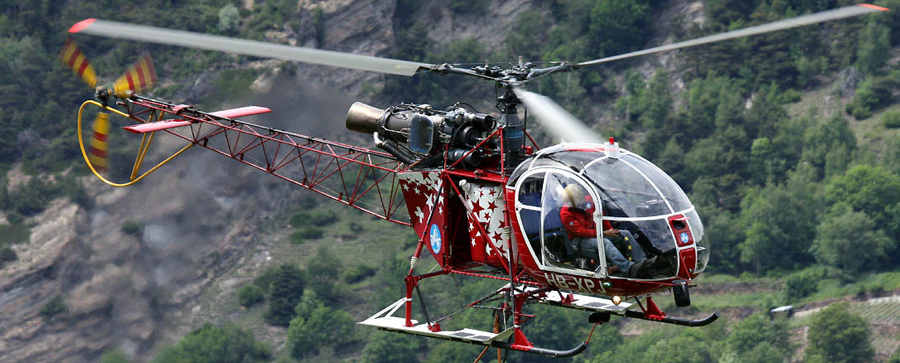
\includegraphics[width=0.95\linewidth]{PICTURES/2_Lama_truss/PNG/lama1.png}
	\end{center}
	\caption {SA-315b Lama helicopter}
\end{figure}
%\vspace{0.5cm}



\clearpage
\subsection*{General structural description }
\addcontentsline{toc}{subsection}{General structural description}
\noindent From the structural point of view the helicopter consists of three main sections: 
\begin{itemize}
	\item the cabin;
	\item the central structure;
	\item the tailboom (which is of our interest).
\end{itemize}

\noindent The central structure joins the cab with tail boom and supports dynamic components such as the turbine, the main transmission as well as commands, hydraulic controls... \\
For the airframe the manufacturer has foreseen tubular structures made of \emph{hermetically welded and interconnected steel tubes}. This solution is excellent for its simplicity and solidity and makes it easy to calculate the forces caused by traction, twist and compression. \\

\medskip
\begin{figure}[h]
	\begin{center}
		\centering  		 		
		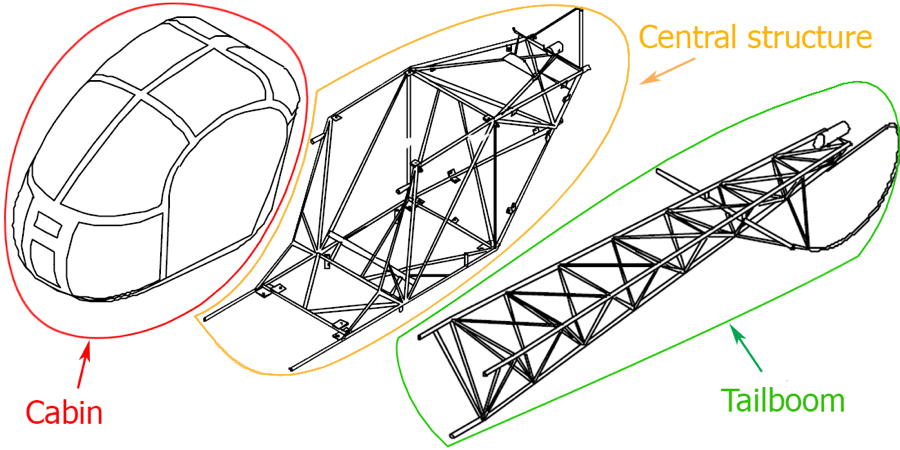
\includegraphics[width=0.8\linewidth]{PICTURES/2_Lama_truss/PNG/structure_parts.png}
	\end{center}
	\caption {Helicopter's main structural sections}
\end{figure}
\vspace{0.5cm}


\noindent INTELLIGENT SOLUTION FOR EASIER STRUCTURAL INSPECTIONS: \

\smallskip
\noindent All the airframes tubes have been designed to be filled with \textbf{Nitrogen gas under pressure} which is periodically measured in order to verify the presence of cracks or damages in some points of the structure. Furthermore, the inert gas prevent the corrosion of the structures caused by the presence of Oxygen. \\
This is undoubtedly a very intelligent and innovative solution for that time and can guarantee the safety of the flight and a long life to all the  airframe's components. \\
However, \underline{the pressure inside the tubes has been neglected in our models} cause its contribution is not so relevant from the structural and dynamical point of view.




\clearpage
\subsection*{Some useful technical specifications}
\noindent
\addcontentsline{toc}{subsection}{Some useful technical specifications}
Some data from official technical sheets and manuals will be here reported cause they have been found to be necessary to characterize some parameters of the Ansys's models and also to verify the validity of some of the obtained results. \\  


\medskip
\begin{figure}[h]
	\begin{center}
		\centering  		 		
		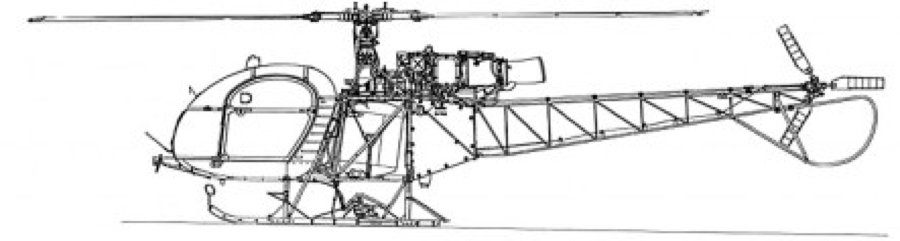
\includegraphics[width=1\linewidth]{PICTURES/2_Lama_truss/PNG/side_view.png}
	\end{center}
	\caption {SA-315b Lama technical drawing}
\end{figure}
%\vspace{0.5cm}

\smallskip
\begin{table}[h!]
	\centering
	
	\begin{tabular}{c c c c} 
		\toprule
		\multicolumn{4}{c}{Helicopter's technical parameters}\\
		\midrule
		Group & Parameter & Value & Description \\
		\midrule
		 & Length & 10.24 $[m]$  & Total helicopter's length \\
		 & Height & 3.09 $[m]$  & Max height of the helicopter \\ 
		Dimensions & $D_{main}$ & 11.02 $[m]$  & Main rotor diameter (3 blade) \\ 
		 & $A_{main}$ & 95.38 $[m^2]$ & Main rotor disk area \\  
		 & $D_{tail}$ &  1.912 $[m]$ & Tail rotor diameter (3 blade) \\ 
		 & $A_{tail}$ & 2.87 $[m^2]$ & Tail rotor disk area \\  
		 
		 
		 \midrule
		 & Max top Power & 640 $[kW]$  & Max take-off power \\
		 Engine & Max continuous Power & 440 $[kW]$  & Max continuous power \\ 
		 & Torque & 398 $[kW]$  & Max torque on transmission \\  
		
		\midrule
		
		 & $N_{engine}$ &  33500 $[RPM]$ & Engine's speed (turbine) \\
		 & $N_{output}$ &  5773 $[RPM]$ & Engine's output drive shaft \\ 
		 Speeds & $N_{rotor}$ &  353 $[RPM]$ & Main rotor normal speed \\
		 & $N_{tailrotor}$  &  2020 $[RPM]$ & Tail rotor normal speed \\ 
		 & $N_{shaft}$ &  5232 $[RPM]$ & Tailrotor's drive shaft speed \\ 
		 
			
		
		\midrule
		& $M_{empty}$ & 1021 $[kg]$  & Empty weight \\
		& $Max_{weight}$ & 2300 $[kg]$  & Max weight (with external load) \\ 
		Masses & $Engine$ & 182 $[kg]$  & Engine weight \\ 
		& $Gearbox$ & 40 $[kg]$ & Tail rotor's gearbox \\  
		& $Tail rotor$ &  25 $[kg]$ & Tail rotor weight \\  
		
		
		
		\bottomrule
	\end{tabular}
	\caption{Lama's technical parameters}
	\label{data}
	
\end{table}











\clearpage
\subsection*{Tailboom's design description (tubular)}
\addcontentsline{toc}{subsection}{Tailboom's design}
\noindent
The SA-315b Lama's tailboom structure is the airframe's part we intend to study. \\
It is composed of a trellis frame of stainless steel tubes welded together to form triangular sections connected by three main longerons that run longitudinally all the tail's length. Dimensions of the triangular sections fade out linearly along the longitudinal direction. \\
The upper horizontal cross members support the tail rotor driving shaft (fixed by bearings to the tail frame) and the tail rotor assembly which basically consist in a gearbox, a rotor hub and the blades with its hinges and actuators for yaw control. \ At the rear end there is an arched bend tube serving as a tail rotor passive protection system which prevents tail rotor from contacts with the ground or with obstacles. 

%three-quarter of the trellis there are two fixed aerodynamic surfaces joined by a transverse tube, which perform the stabilizer function during the forward flight, while at the rear

\begin{figure}[h]
	\begin{center}
		\centering  		 		
		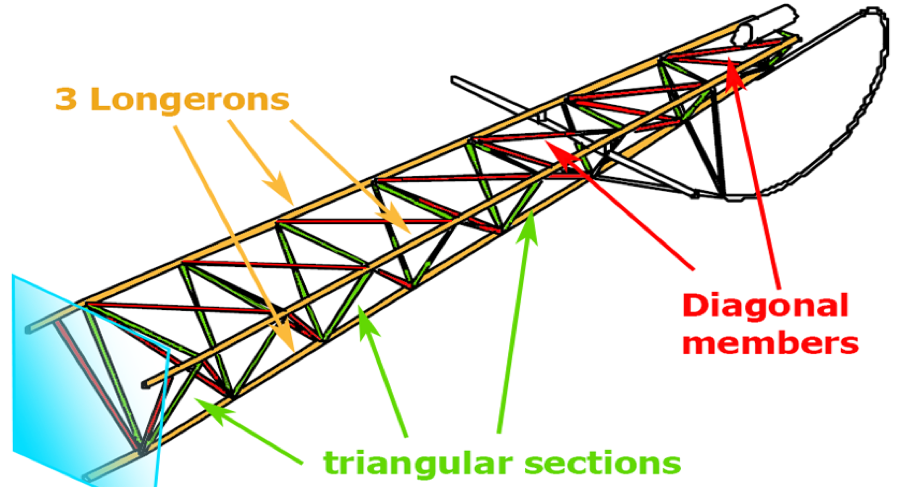
\includegraphics[width=1\linewidth]{PICTURES/2_Lama_truss/PNG/tail_written.png}
	\end{center}
	%\caption {Lama tailboom's section}
\end{figure}
%\vspace{0.5cm}

\section*{Material properties}
\noindent
Elastic isotropic materials are used in the FE model. As previously outlined, the SA315b tailboom's frame is made of staineless steel tubes welded together at the joints. The properties of the steel used for the calculations are listed in the table:

\medskip
\begin{table}[h!]
	\centering
	
	\begin{tabular}{c c c c} 
		\toprule
		\multicolumn{4}{c}{Material properties}\\
		\midrule
		Mat & Density (kg/m3) & Poisson's ratio & Young's modulus (GPa) \\
		\midrule
		Steel & 7850  &  0.29 & 205 \\ 
		\bottomrule
	\end{tabular}	
\end{table}


\clearpage
\subsection*{Tubes real constants and properties}
\addcontentsline{toc}{subsection}{Tubes real constants and material properties}

\noindent
Airframe's tubes have all been modelled using BEAM elements with hollow circle cross sections (CTUBE) which have different real constants depending on type of the tube. \\ Property of the sections used in the model as well as the formula used to perform the calculations are listed in the following tables. 

\bigskip
\begin{figure}[h]
	\begin{center}
		\centering  		 		
		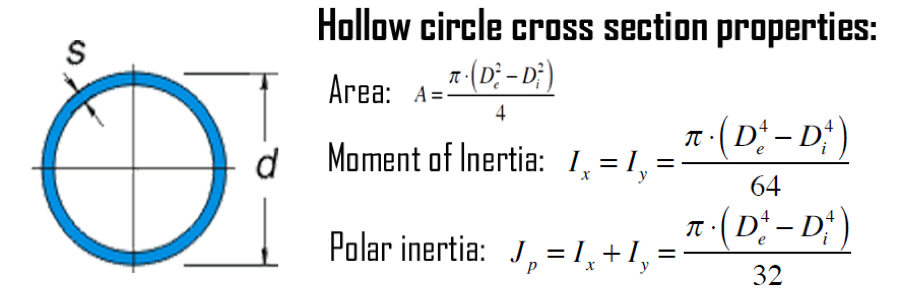
\includegraphics[width=0.9\linewidth]{PICTURES/2_Lama_truss/PNG/tube1.png}
	\end{center}
	\caption {Tube's cross section}
\end{figure}
%\vspace{0.5cm}


\medskip
\begin{table}[h!]
	\centering
	
	\begin{tabular}{c c c c} 
		\toprule
		\multicolumn{4}{c}{Tubes cross section's properties}\\
		\midrule
		Family & Parameter & Value & Description \\
		\midrule
		& $\phi_{ext}$ &  \textbf{28} $[mm]$ & External diameter \\
		& $s$ &  \textbf{2} $[mm]$ & Tube's thickness \\ 
		Longerons & $A_{section}$  &  163 $[mm^2]$ & Area of the cross section \\ 
		& $I_{x} = I_{y}$ &  $13885.8$ $[mm^4]$ & Moment of inertia \\ 
		& $I_{p}$ &  $6942.9$ $[mm^4]$ & Polar moment of inertia \\
		

		\midrule
		& $\phi_{ext}$ &  \textbf{12} $[mm]$ & External diameter \\
		& $s$ &  \textbf{1.5} $[mm]$ & Tube's thickness \\ 
		Cross elements & $A_{section}$  &  49.5 $[mm^2]$ & Area of the cross section \\ 
		& $I_{x} = I_{y}$ &  $695.8$ $[mm^4]$ & Moment of inertia \\ 
		& $I_{p}$ &  $347.9$ $[mm^4]$ & Polar moment of inertia \\
		
		
		\midrule
		& $\phi_{ext}$ &  \textbf{12} $[mm]$ & External diameter \\
		& $s$ &  \textbf{1.5} $[mm]$ & Tube's thickness \\ 
		Diagonal elements & $A_{section}$  &  49.5 $[mm^2]$ & Area of the cross section \\ 
		& $I_{x} = I_{y}$ &  $695.8$ $[mm^4]$ & Moment of inertia \\ 
		& $I_{p}$ &  $347.9$ $[mm^4]$ & Polar moment of inertia \\
		
			
		\bottomrule
	\end{tabular}
	\caption{Tailboom's technical parameters}
	
\end{table}

\noindent
In this case it is possible to use the default generalized cross-sections included in the Ansys "SECTYPE" command of the beam elements.




\clearpage
\section*{Approach to the problem}
\section{Basic structure model (airframe only)}
\subsection*{Analysis model}
\addcontentsline{toc}{subsection}{Analysis model}
\noindent
A fully parametric model of the truss tail boom has been developed in Ansys APDL language on the base of the technical drawings found on the aircraft's official manuals and reported in the appendix. Some missing dimensions have been recovered from a scaled CAD model of the same helicopter type developed by model aircraft's builders. \\
The model has been developed using a \emph{bottom-up approach} creating the necessary key-points and lines and then meshing the elements. Additional local reference frames have been used to simplify the geometry definition. \\
The following picture outline the main features of the naked structure's model. \\

 \medskip
 \begin{figure}[h]
 	\begin{center}
 		\centering  		 		
 		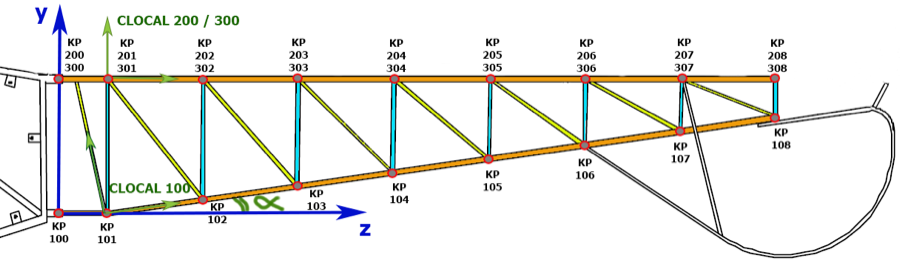
\includegraphics[width=1\linewidth]{PICTURES/2_Lama_truss/PNG/tail_complete_mod.png}
 	\end{center}
 	\caption {Tailboom's analysis model (truss)}
 \end{figure}
 %\vspace{0.5cm}
 
 \bigskip
 \begin{table}[h!]
 	\centering
 	
 	\begin{tabular}{c c c} 
 		\toprule
 		\multicolumn{3}{c}{Tailboom's main parameters}\\
 		\midrule
 		Parameter & Value & Description \\
 		\midrule
 		Lt & 4.8 $[m]$  & Total tail length \\
 		L1 & 0.7 $[m]$  & Equilateral triangular section side lenght (at the root) \\ 
 		L5 & 0.075 $[m]$  & Half width of the tail at the tip (along x axis) \\ 
 		w1 & 0.48 $[m]$ & z-coordinate of KP 101 (Lt/10) \\  
 		alpha &  10 $[deg]$ & Angle of inclination of the lower longeron \\

 		\bottomrule
 	\end{tabular}
 	\caption{Problem's data}
 	
 \end{table}

\clearpage
\subsection*{Model assumptions}
\addcontentsline{toc}{subsection}{Model assumptions}

\noindent
\begin{quoting}
	\begin{itemize}
		
		\item Element type: \textbf{BEAM 189}, a quadratic 3-node element in 3D with 6 dofs for each node and based on Timoshenko beam theory which includes shear-deformation effects;
		
		\item uniform cross-sections of the elements along the tail's length;
		
		\item \underline{linear elastic isotropic} material properties;
		
		\item self-weight of the elements considered;
		
		\item geometrical non-linearities included in the static analysis (NLGEOM,ON) \\
		
	\end{itemize}
\end{quoting}

 \smallskip
\subsection*{Tailboom model (airframe only)}

\begin{figure}[h]
	\begin{center}
		\centering  		 		
		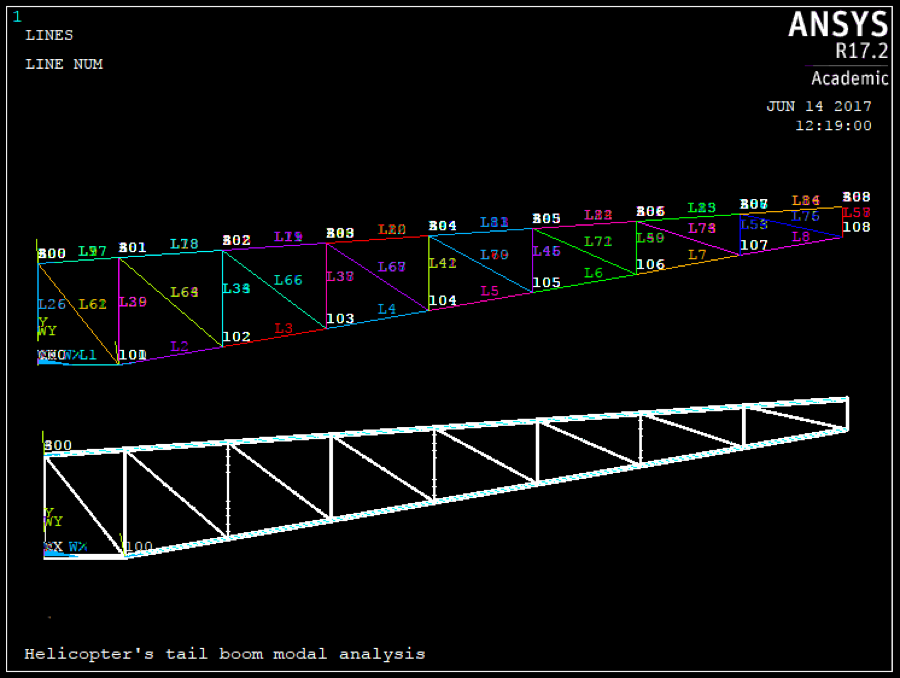
\includegraphics[width=1\linewidth]{PICTURES/2_Lama_truss/PNG/model_1_mod.png}
	\end{center}
	\caption {Analysis model (truss) side view}
\end{figure}
\vspace{0.5cm}



\noindent
Isometric views of the model in which it is possible to see the keypoints generated and the lines representing the beam's axes as well as the resulting elements. 
 \smallskip
\begin{figure}[h!]
	\begin{center}
		\centering  		 		
		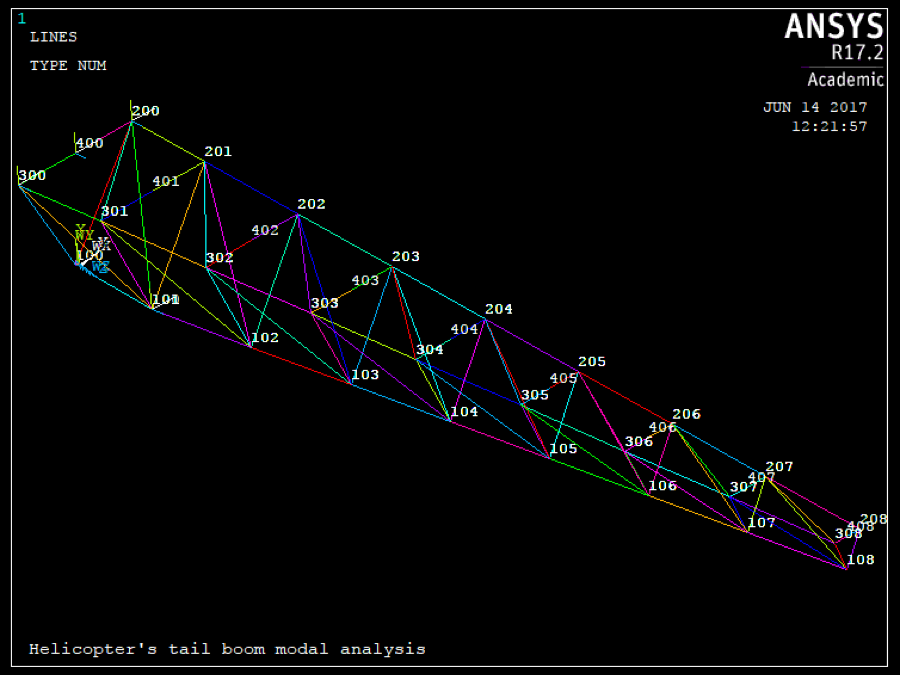
\includegraphics[width=0.79\linewidth]{PICTURES/2_Lama_truss/PNG/model_2.png}
	\end{center}
	\caption {Structure of the model - (3D view)}
\end{figure}
%\vspace{0.5cm}

\smallskip
\begin{figure}[h!]
	\begin{center}
		\centering  		 		
		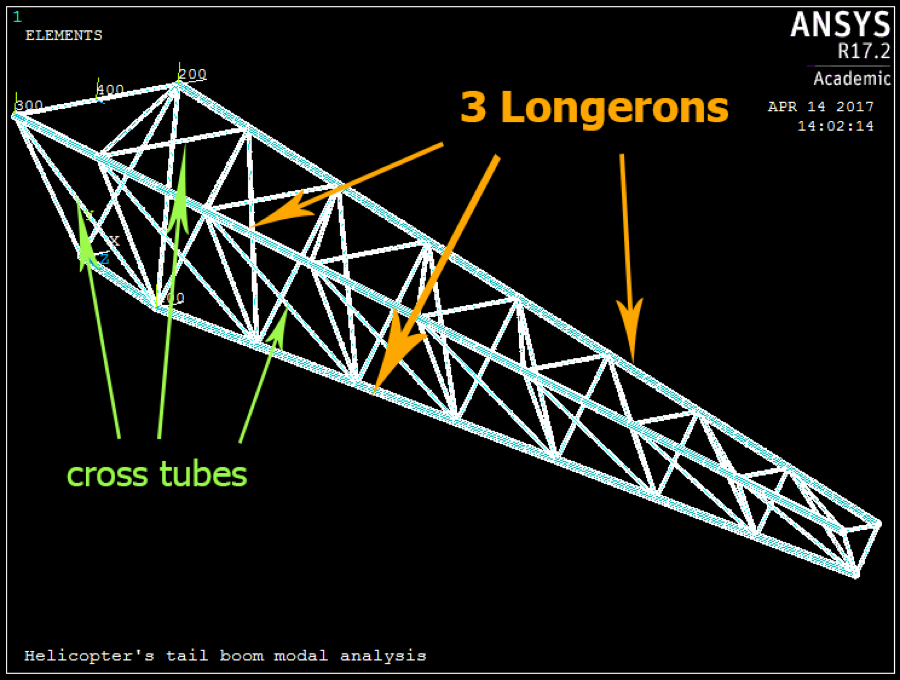
\includegraphics[width=0.79\linewidth]{PICTURES/2_Lama_truss/PNG/beam_ISO2.png}
	\end{center}
\end{figure}
%\vspace{0.5cm}
 


\clearpage
\subsection*{Applied loads for static analysis}
\addcontentsline{toc}{subsection}{Applied loads for static analysis}
\noindent
To verify the model by means of a preliminary static analysis we just considered the effect of the \textbf{self-weight} of the structure and the contribution of the \textbf{thrust (Ty)} which is provided by the tail rotor to balance the maximum applied torque by the motor. 

\smallskip
\begin{figure}[h!]
	\begin{center}
		\centering  		 		
		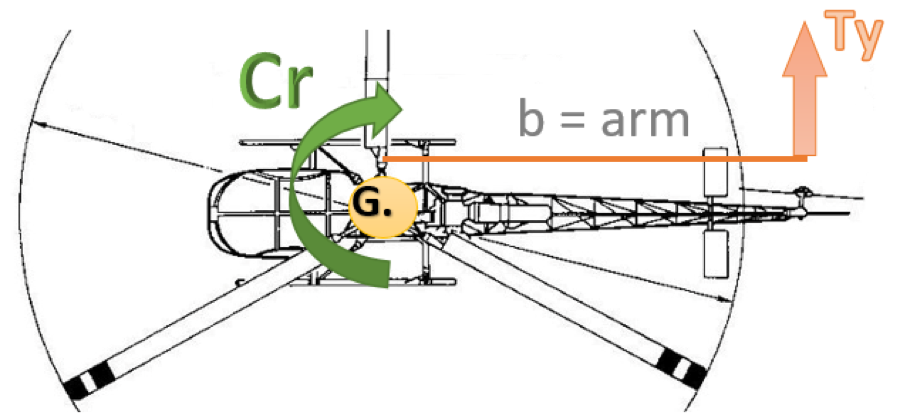
\includegraphics[width=0.79\linewidth]{PICTURES/2_Lama_truss/PNG/anticoppia.png}
	\end{center}
\end{figure}
%\vspace{0.5cm}

\noindent
ASSUMPTIONS: 
\begin{itemize}
	\item Ty is orthogonal to the plane of rotation of the tail rotor;
	\item It is computed from helicopter's technical data considering its maximum value corresponding to the maximum torque applied to the main rotor by the transmission;
	\item Cr is the reaction torque equal to the Cm (maximum motor torque) because of the third newton law. 
	\item Aerodynamic forces, inertial and centrifugal accelerations due to manoeuvres during flight are not taken into account.
\end{itemize}

\noindent
The equations used to compute the value of the force are:
\begin{equation*}
Torque (N*m) \, \, = \, \, \frac{Power \, \, absorbed(W)}{head \, \, speed(rad/s)}  
\end{equation*}

\begin{equation*}
C_m  = \frac{W}{\omega} \, = \, \frac{398000 (W)}{36.966 (rad/s)} \, = \, 10767 (Nm)
\end{equation*}
where W is the main rotor maximum power absorbed, while $\omega$ is the main rotor head speed. \
The tail rotor thrust required can be computed from the following eq. :

\begin{equation*}
C_r = T_y * b \, \, \, \, \, => \, \, \, \, \,  Ty = \frac{C_r}{b} \, = \, \frac{10767(Nm)}{4.8 (m)}  \, = \, \textbf{2243} \, (N)
\end{equation*}



\clearpage
\subsection*{Applied boundary conditions}
\addcontentsline{toc}{subsection}{Applied boundary conditions}
\noindent
According to the literature, helicopter's vibrations, caused by the main rotor assembly, are usually analyzed by assuming the response of the fuselage to react in a similar manner to that of a 'free-free' beam. \\
However, our interest is limited at the study of a part of the entire structure, the tailboom; this requires a different investigation procedure. \\ 
For the project's purposes, the tail boom can be satisfactorily modelled as a beam structure which is rigidly clamped at the large cockpit mass so it can be seen as a fixed-free beam. \\





\smallskip
\begin{figure}[h!]
	\begin{center}
		\centering  		 		
		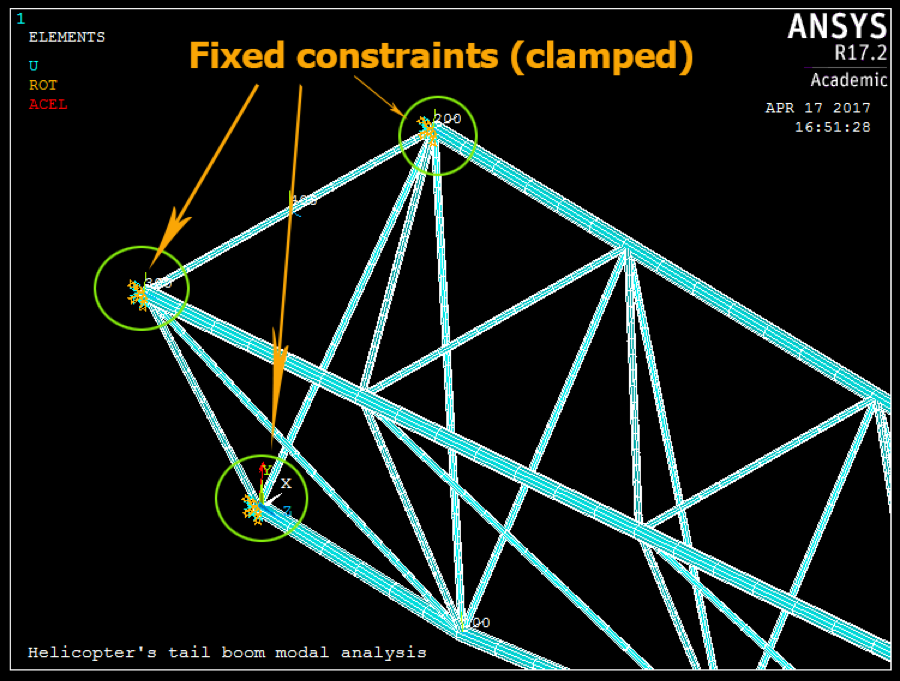
\includegraphics[width=0.8\linewidth]{PICTURES/2_Lama_truss/PNG/BC.png}
	\end{center}
	%\caption{Model's boundary conditions}
\end{figure}	
%\vspace{0.5cm}

\smallskip
\begin{figure}[h!]
	\begin{center}
		\centering  		 		
		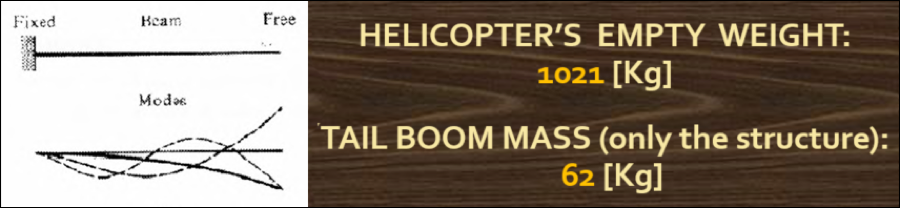
\includegraphics[width=1\linewidth]{PICTURES/2_Lama_truss/PNG/BC1.png}
	\end{center}
\end{figure}	
%\vspace{0.5cm}

\noindent
NODES AT THE ROOT of the tail -> ALL dofs (displacements and rotations) locked; \\
TAIL ROTOR THRUST FORCE -> applied at the tail tip node and acts orthogonally.


\clearpage
\subsection*{Preliminary static solution (model checking)}
\addcontentsline{toc}{subsection}{Preliminary static solution}
\noindent
At the very beginning, a preliminary static analysis has been done in order to check the \textbf{effectiveness} of the FEM model developed. 
In this step, geometrical non-linearities (stress-stiffening effects) has been included (command "NLGEOM,ON") and the optimized default options to find the non linear solutions has been also activated ("SOLCONTROL,ON"). After this step, the model is ready to be solved.

\subsubsection*{PLDISP and PLNSOL (node's displacement)}
%\smallskip
\begin{figure}[h!]
	\begin{center}
		\centering  		 		
		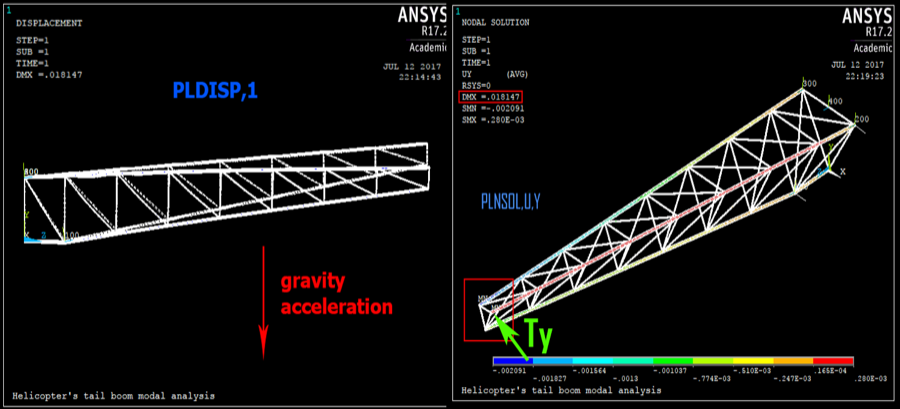
\includegraphics[width=0.95\linewidth]{PICTURES/2_Lama_truss/PNG/displ.png}
	\end{center}
	%\caption{Model's boundary conditions}
\end{figure}	
%\vspace{0.5cm}

\subsubsection*{Reactions at constrained nodes PRRSOL}
%\smallskip
\begin{figure}[h!]
	\begin{center}
		\centering  		 		
		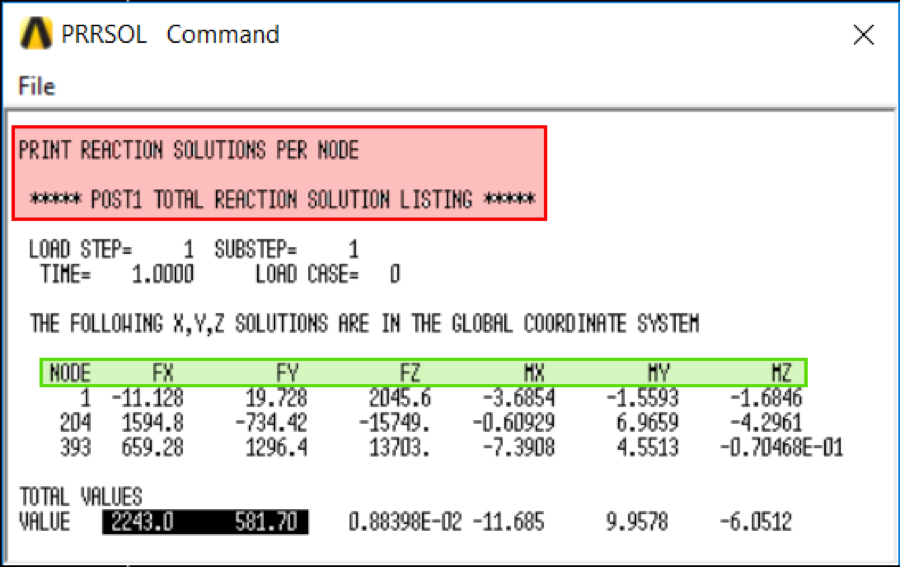
\includegraphics[width=0.65\linewidth]{PICTURES/2_Lama_truss/PNG/PRRSOL.png}
	\end{center}
	%\caption{Model's boundary conditions}
\end{figure}	
%\vspace{0.5cm}
\noindent
Results match with the self-weight (vertical) and the tail thrust (horizontal) forces applied. 
\clearpage



\clearpage
\section*{Modal Analysis (airframe only)}
\addcontentsline{toc}{subsection}{Modal Analysis (airframe only)}
\noindent
Modal analysis is a technique used to determine the structure's vibration characteristics (vibration modes) in terms of \textbf{natural frequencies}, \textbf{modal shapes} and eventually \textbf{mode partecipation factors}. \\
This is one of the project's scopes aimed to dynamically characterize the structure. \\

\noindent
\underline{ASSUMPTIONS}:
\begin{itemize}
	\item free vibration (forces, pressures...are ignored in modal analysis);
	\item no damping (it effect on $\omega_{n}$ is negligible);
	\item synchronous harmonic motions.  
\end{itemize}

\smallskip
\noindent
The approach consists to solve an EIGENVALUE PROBLEM in order to compute the resonant frequencies (eigenvalues) and modal shapes (eigenvectors) of the characteristic polynomial by means of \emph{suitable algorithms}. 

\medskip
\begin{figure}[h!]
	\begin{center}
		\centering  		 		
		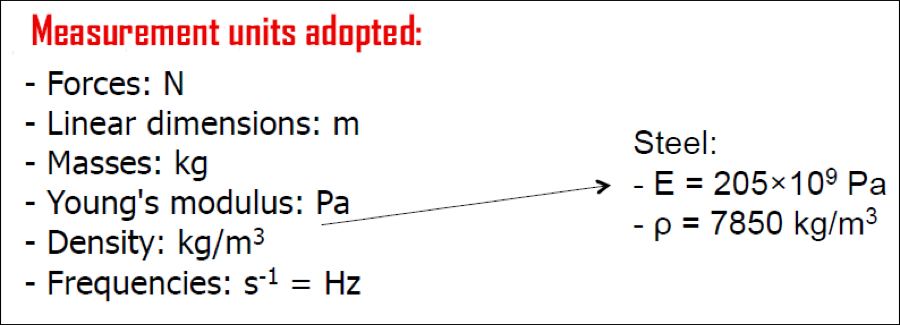
\includegraphics[width=0.8\linewidth]{PICTURES/2_Lama_truss/PNG/MU.png}
	\end{center}
	\caption{Note on measurement units adopted}
\end{figure}	
%\vspace{0.5cm}

%\smallskip
\begin{figure}[h!]
	\begin{center}
		\centering  		 		
		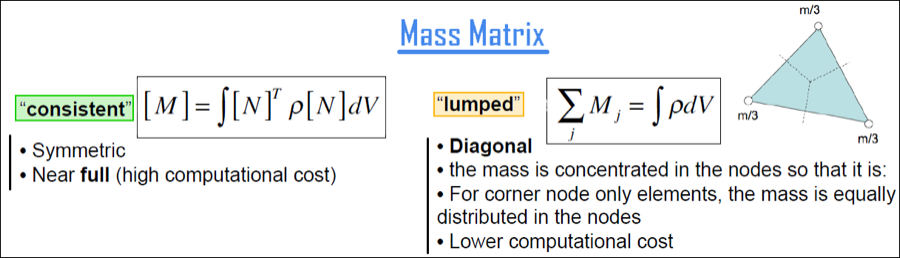
\includegraphics[width=1\linewidth]{PICTURES/2_Lama_truss/PNG/CL1.png}
	\end{center}
	\caption{Note on consistent and lumped mass matrix formulation}
\end{figure}	
%\vspace{0.5cm}


\clearpage
\subsubsection*{Note on the real tubes masses}
\noindent
The shapes and frequencies are directly dependent on the mass and stiffness properties of the elements of the structure. Hence, the masses of the tubes are an important parameter in the computations regarding the modal analysis. To be accurate in modelling, the real \emph{weight per meter mass} of the tailboom's tubes have been found from the manufacturer and have been loaded as a material parameter using the ADDMASS option of the beam elements SECCONTROL command that allows to specify the value of the real weight of the tubes per unit length. 

\subsubsection*{Model checking}
\noindent
The total mass of the taiboom frame has been computed from the Ansys model in order to check the consistency of the model developed with respect to the real aircraft's data. \\
The value of the mass of the taiboom without the additional subsystems results in 62.5 kg which matches the expected mass estimated from the real technical data.
\begin{figure}[h]
	\begin{center}
		\centering  		 		
		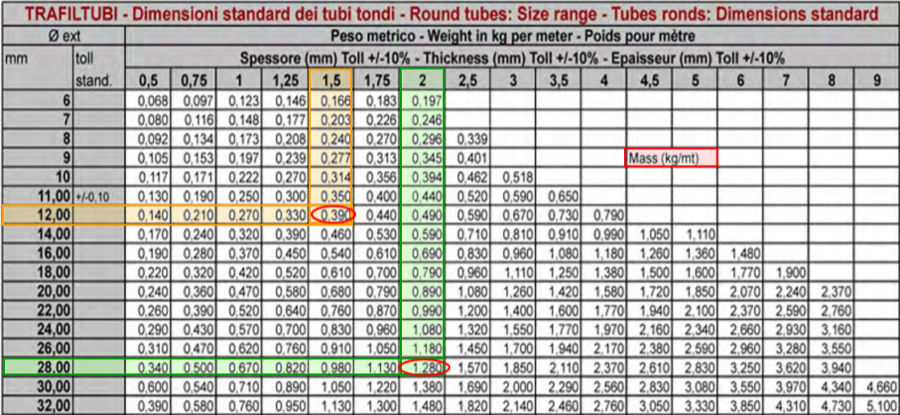
\includegraphics[width=1\linewidth]{PICTURES/2_Lama_truss/PNG/addmass2.png}
	\end{center}
	\caption {Tubes weight per unit length}
\end{figure}
%\vspace{0.5cm}




\begin{figure}[h]
	\begin{center}
		\centering  		 		
		
\includegraphics[width=0.8\linewidth]{PICTURES/2_Lama_truss/PNG/tot_mass.png}
	\end{center}
	\caption {Tubes weight per unit length}
\end{figure}
%\vspace{0.5cm}


\clearpage
\subsection*{Analysis type and options}
\noindent
\begin{figure}[h]
	\begin{center}
		\centering  		 		
		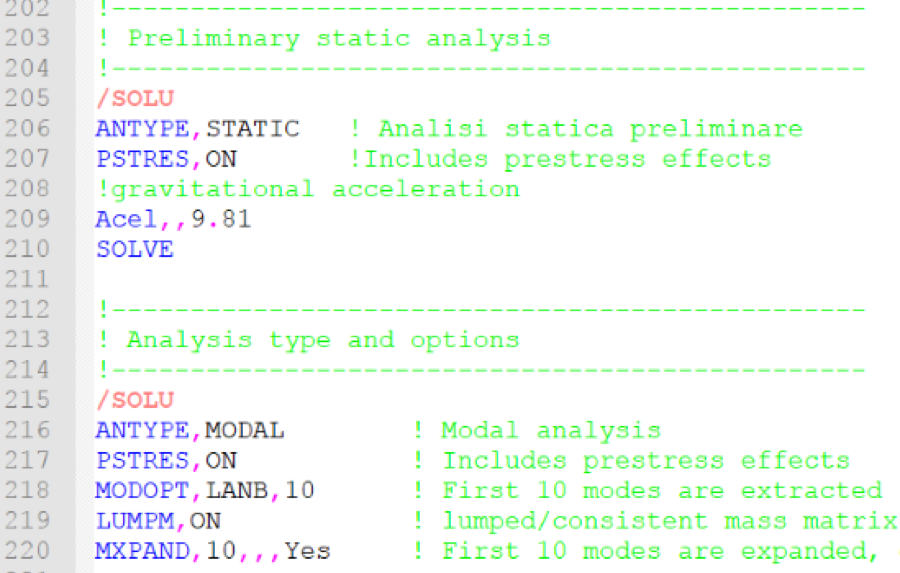
\includegraphics[width=0.9\linewidth]{PICTURES/2_Lama_truss/PNG/antype2.png}
	\end{center}
\end{figure}


\subsection*{Convergence analysis}
\noindent
\begin{figure}[h]
	\begin{center}
		\centering  		 		
		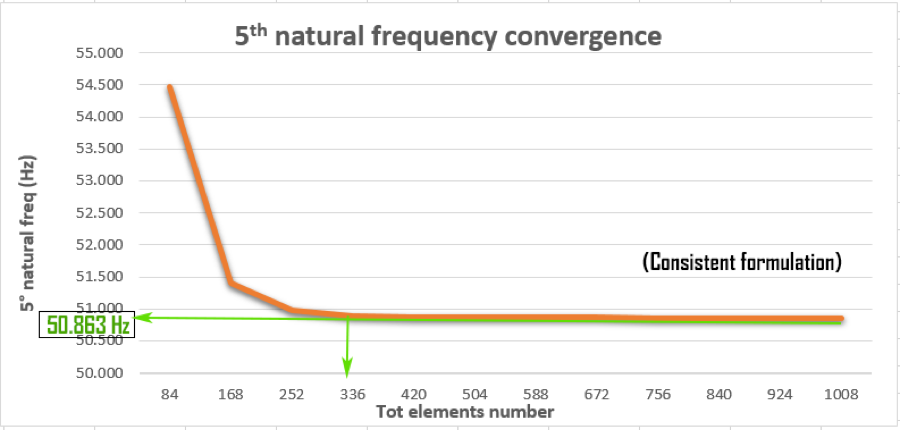
\includegraphics[width=0.8\linewidth]{PICTURES/2_Lama_truss/PNG/cov.png}
	\end{center}
	\caption {Convergence analysis on the 5th natural frequency}
\end{figure}



\subsection*{Resonant frequencies}
\noindent
The first 10 resonant frequencies obtained at the end of the convergence analysis are now displayed in the following results table:
\begin{figure}[h]
	\begin{center}
		\centering  		 		
		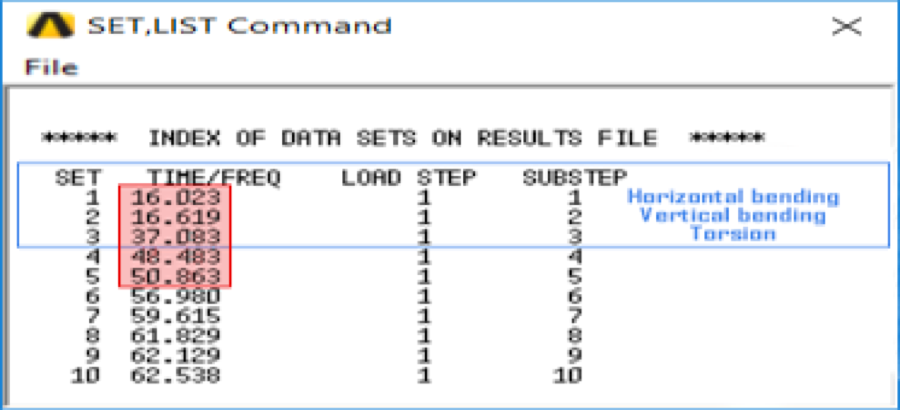
\includegraphics[width=0.70\linewidth]{PICTURES/2_Lama_truss/PNG/set-list.png}
	\end{center}
	%\caption {List the first 10 computed natural frequencies}
\end{figure}

\subsection*{First 4 modal shapes}
\noindent
Eigenvectors are typically normalized in Ansys with respect to the mass matrix and; this normalization is very useful from the computational point of view. However, the drawback is that in this way they represent correctly the shape of the mode but not the real amplitude of the displacement which in turn depends on the initial conditions. 

\begin{figure}[h]
	\begin{center}
		\centering  		 		
		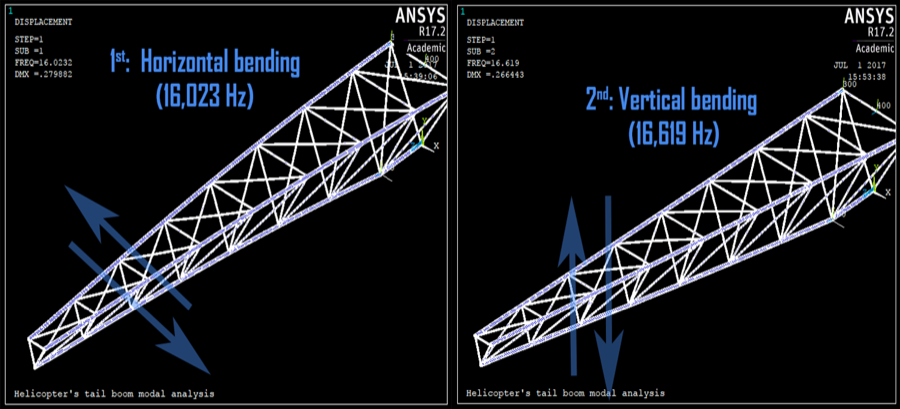
\includegraphics[width=0.95\linewidth]{PICTURES/2_Lama_truss/PNG/1-2.png}
	\end{center}
	\caption {Graphical representation of the first and second modal shapes}
\end{figure}

\noindent
The first three mode shapes are related to the \emph{horizontal,vertical and torsional} movement of the tailboom. The fourth shows a node at the rear three quarter of the tail while higher order modes are related to tubes movements at higher frequencies. 

\begin{figure}[h]
	\begin{center}
		\centering  		 		
		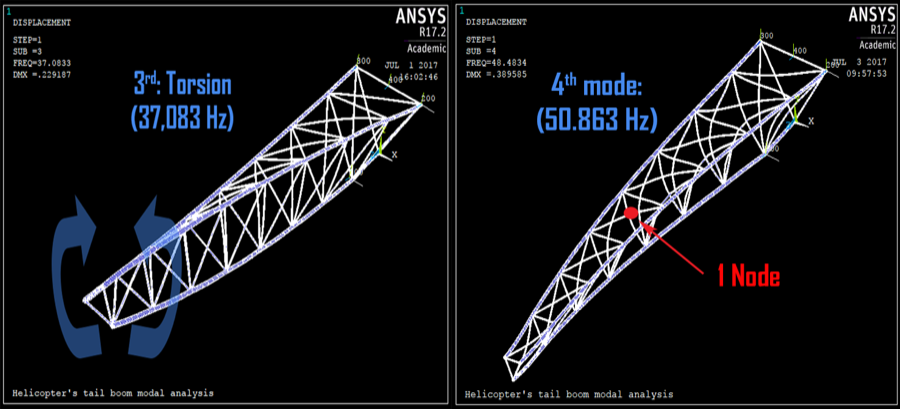
\includegraphics[width=0.95\linewidth]{PICTURES/2_Lama_truss/PNG/3-4.png}
	\end{center}
	\caption {Graphical representation of the third and fourth modal shapes}
\end{figure}


%\clearpage
\subsection*{Results comparison with literature}
\noindent
In order to have a reference about the results obtained from Ansys, our computed tailboom's natural frequencies have been compared with those found in the literature. Serendipitously, dimensions and materials of the helicopter's model analyzed in the paper are comparable to our model and also the results found at the end of the convergence analysis reasonably match with those reported in the literature (maximum 5 \% difference) at least for the first three vibration modes. \\
\begin{figure}[h]
	\begin{center}
		\centering  		 		
		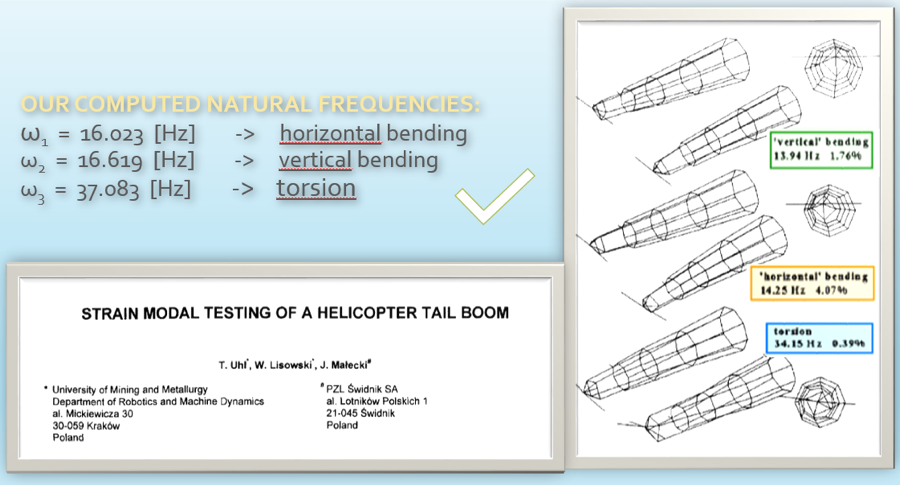
\includegraphics[width=1\linewidth]{PICTURES/2_Lama_truss/PNG/comparison.png}
	\end{center}
	%\caption {Results comparison with literature data found}
\end{figure}

\clearpage
\section{Fully parametric model (airframe + subsystems)}
\noindent
At this point only the naked tailboom's airframe has been studied. It is necessary to model also the subsystems fixed on it in order to perform an accurate characterization of the dynamic behaviour of the whole real system. \\
The additional components present on an helicopter tail are basically:
\begin{itemize}
	\item the \underline{tail rotor's driving shaft} and the bearings that support it;
	\item the tail rotor assembly composed of the \underline{rotor hub}, \underline{blades} and the 90 degrees \underline{gearbox};
	\item aerodynamic surfaces such as the \underline{horizontal stabilizers};
	\item an \underline{arched bend tube} serving as a tail rotor passive protection system.
\end{itemize}



\smallskip
\begin{figure}[h!]
	\begin{center}
		\centering  		 		
		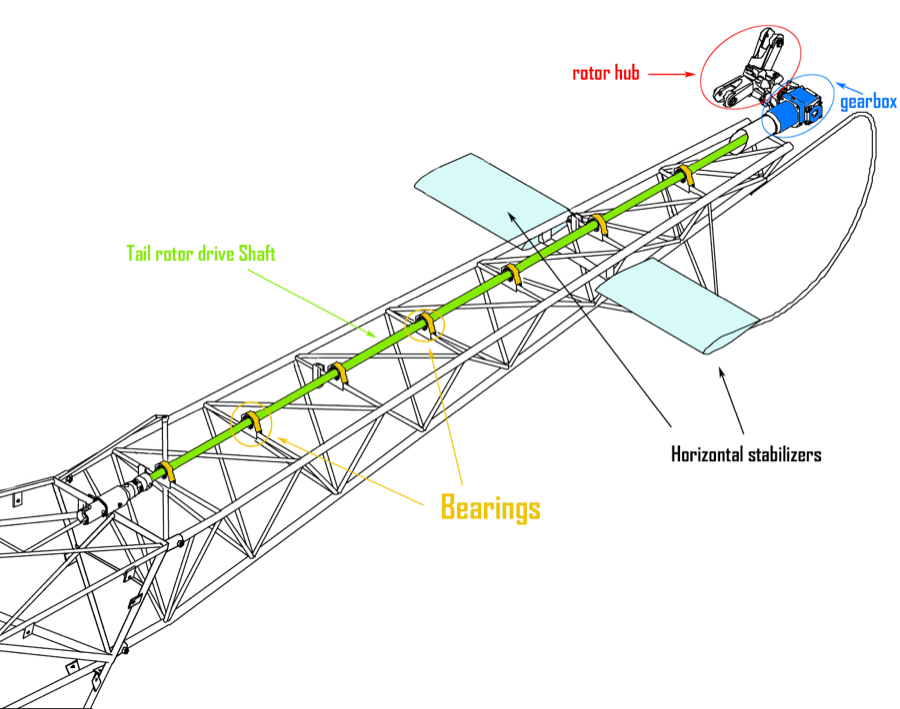
\includegraphics[width=1\linewidth]{PICTURES/2_Lama_truss/PNG/model2/tail_complete_2.png}
	\end{center}
	%\caption{Additional subsystems}
\end{figure}	
%\vspace{0.5cm}

\noindent
For our purposes, the horizontal stabilizers have been considered only as concentrated masses neglecting the aerodynamic forces they produce since we are considering a stationary (hover) fly condition whereas the rotor protection tube has been, instead, neglected. 

\clearpage
\subsection*{Tail rotor's drive shaft}
\noindent
The Tail Rotor drive system receives the energy from the engine and consists in two parts (a forward drive shaft attached directly to the engine and a longer rear drive shaft) which are both connected to each other, to the engine and to the Tail Gear Box by 3 \emph{flexible couplings} to allow lateral and vertical motions of the tailboom. \\
The very long tail rotor drive shaft is supported by 7 ball bearing support assemblies mounted on rubber bushes that damp out the vibrations.

\smallskip
\begin{figure}[h!]
	\begin{center}
		\centering  		 		
		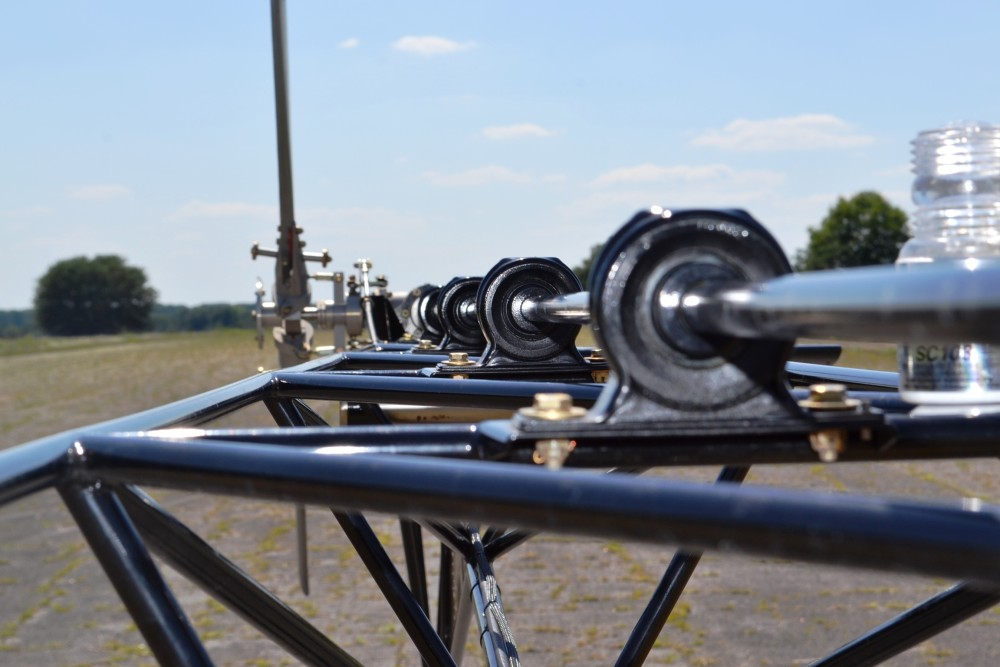
\includegraphics[width=0.85\linewidth]{PICTURES/2_Lama_truss/PNG/model2/driveshaft}
	\end{center}
	\caption{Tail rotor drive shaft bearing supported}
\end{figure}	
%\vspace{0.5cm}

\medskip
\begin{table}[h!]
	\centering
	
	\begin{tabular}{c c c c c} 
		\toprule
		\multicolumn{5}{c}{Shaft's properties}\\
		\midrule
		Material & type & Density (kg/m3) & Poisson's ratio & Young's modulus (GPa) \\
		\midrule
		Ergal & serie 7075 & 2810  &  0.33 & 72 \\ 
		\midrule
		\\
		\midrule
		Part & length (m) &   & N° of segments & dimension (m) \\
		\midrule
		Entire shaft length & 4.8 &   & 8  &  0.6  \\ 
		\bottomrule
	\end{tabular}	
\end{table}

\noindent 
The shaft's mass is about 7 kg; however, considering bearings, flexible joints and additional components to fix the shaft along the tail's length, the total mass rises up to \textbf{12 kg} which are considered equally distributed on the 7 point masses located along the tail.
\clearpage
\subsection*{Gearbox}
\noindent
The Tail Gear Box is basically an angle reduction gear for mounted in and protected by a steel casing filled with oil for lubrication purpose. Its weight is around \textbf{30 kg}. \
The transmission ratio is about 2.59 and it contributes to reduce the rotational speed from 5232 RPM of the shaft to the 2020 RPM of the tail rotor hub. \\
The gearbox is connected to the tail boom structure by 3 bolts and which \emph{represent the main interface from which forces, moments and displacements are transferred}. \\

\smallskip
\begin{figure}[h!]
	\begin{center}
		\centering  		 		
		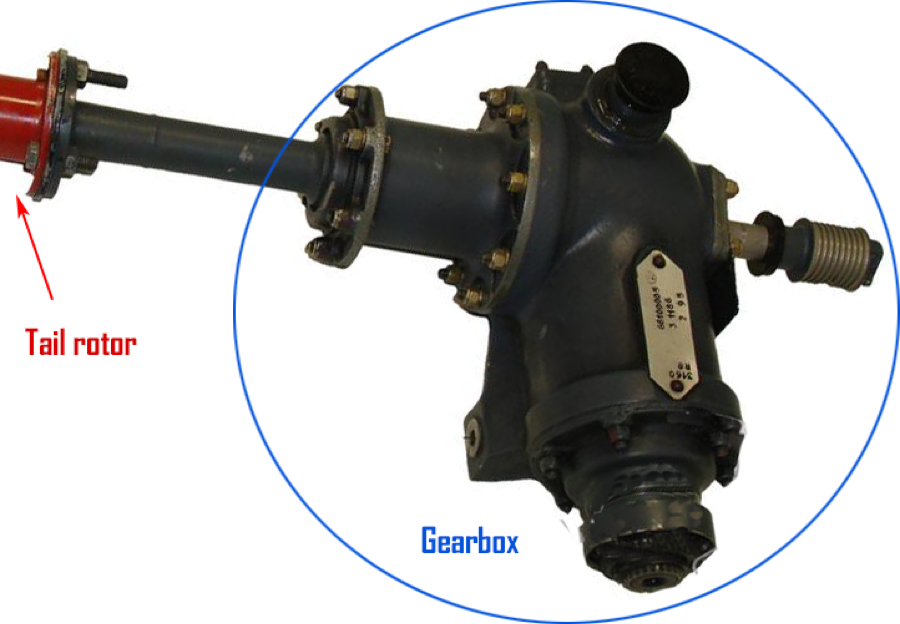
\includegraphics[width=0.8\linewidth]{PICTURES/2_Lama_truss/PNG/model2/gearbox}
	\end{center}
	\caption{90 degrees gearbox}
\end{figure}	
%\vspace{0.5cm}

\medskip
\begin{figure}[h!]
	\begin{center}
		\centering  		 		
		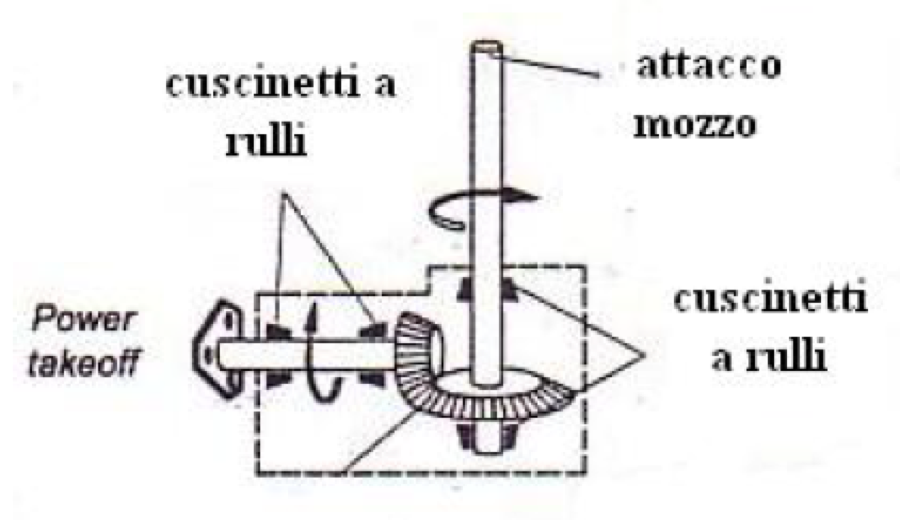
\includegraphics[width=0.65\linewidth]{PICTURES/2_Lama_truss/PNG/gearbox_tail_scheme}
	\end{center}
	%\caption{90 degrees gearbox}
\end{figure}	
%\vspace{0.5cm}


\bigskip
\subsection*{Rotor assembly (hub + blades)}
\noindent
The rotor assembly is composed of a \underline{rotor hub}, \underline{3 blades} and a \underline{shaft} which is connected to the gearbox from one side and it sustain the hub and the blades on the other end. 

\medskip
\begin{table}[h!]
	\centering
	
	\begin{tabular}{c c c c c} 
		\toprule
		\multicolumn{5}{c}{Rotor's assembly properties}\\
		\midrule
		Item & components & Mass (kg) & Polar inertia (kg $m^2$) & Length (m) \\
		\midrule
		Hub & 1 & 30  &  1.776  & / \\ 
		\midrule
		Blades & 3 & 5 each  & / & 0.596 \\
		\midrule
		Shaft & 1 & 1  &  /  & 0.5 \\
		
		\bottomrule
	\end{tabular}	
\end{table}


\smallskip
\begin{figure}[h!]
	\begin{center}
		\centering  		 		
		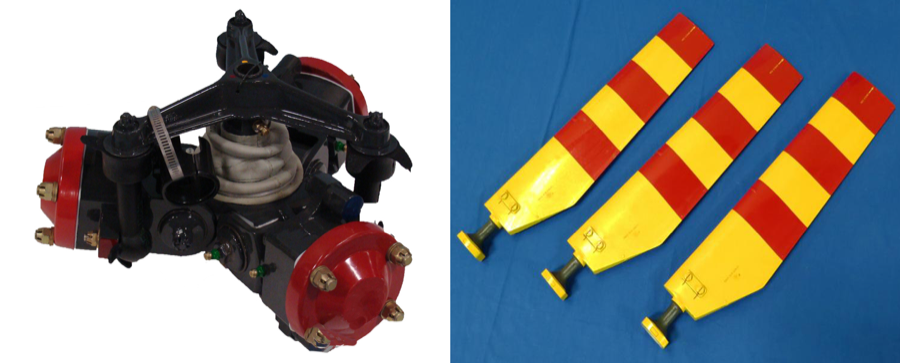
\includegraphics[width=0.9\linewidth]{PICTURES/2_Lama_truss/PNG/model2/hubeblades}
	\end{center}
	\caption{Tail rotor hub and blades}
\end{figure}	
%\vspace{0.5cm}

\subsubsection*{Rotor's concentrated inertia}
\noindent
Blades are modelled as thin rectangular beams ( $I_{blade} = \frac{1}{12} m L^2 $ w.r.t its center of mass).
To consider the inertia respect to the root of the blade, we can use Huygens-Steiner theorem:
\begin{equation*}
I_{root} = I_{CoM} + m_{blade}  \left( \frac{L}{2} \right) ^2  \, = \, 0.59 \, \, (kg \, m^2)
\end{equation*}

\begin{equation*}
I_{rotor} = n_{blades} * I_{root} \, = \,  \textbf{1.776} \, \, (kg \, m^2)
\end{equation*}

\noindent
In literature, as first approximation, tail rotor is considered as a rigid disk fixed on a beam's shaft supported by two elastic bearings. \\
For our purposes, the tail rotor assembly has been modelled considering the \underline{rotor hub} as a \textbf{concentrated mass and inertia} located at the shaft's tip node.




\clearpage
\section*{Modal Analysis (complete model)}
\addcontentsline{toc}{subsection}{Modal Analysis (complete model)}

\begin{figure}[h!]
	\begin{center}
		\centering  		 		
		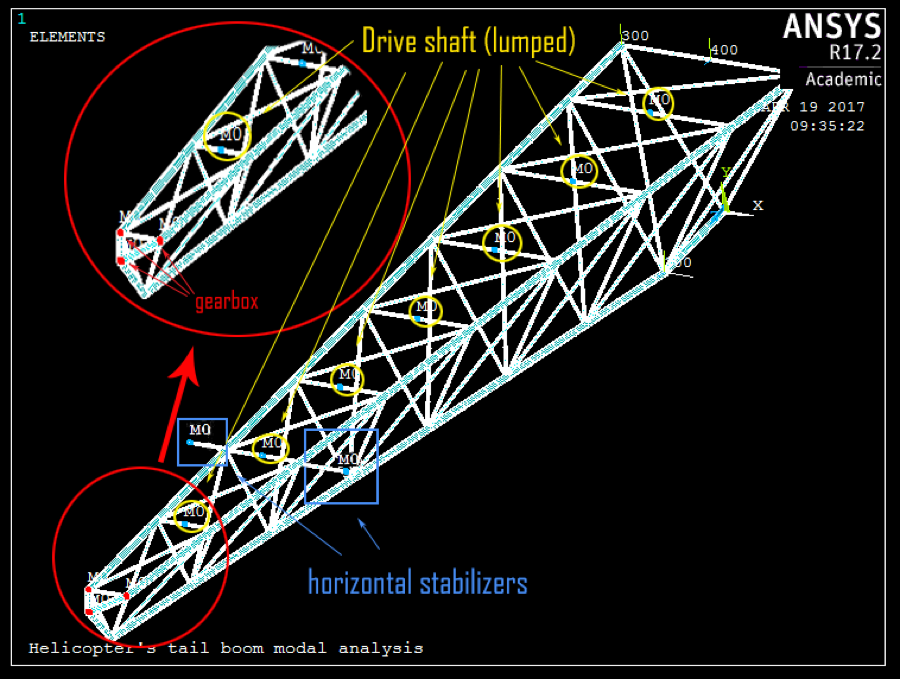
\includegraphics[width=0.9\linewidth]{PICTURES/2_Lama_truss/PNG/model2/lumped_approach1.png}
	\end{center}
	\caption{Additional subsystems}
\end{figure}	
%\vspace{0.5cm}



\subsection*{Applied boundary conditions}
\addcontentsline{toc}{subsection}{Applied boundary conditions}
\noindent
The helicopter structure can be modelled to first approximation as a large point mass (the main rotor assembly and cockpit) connected by the relatively slender tail boom to a small point mass (the tail rotor assembly). Because of this significant difference in mass, the tail boom can be satisfactorily modelled as a beam structure which is rigidly clamped at the large cockpit mass and has an end mass equal to that of the tail rotor assembly. \\

\smallskip
\begin{figure}[h!]
	\begin{center}
		\centering  		 		
		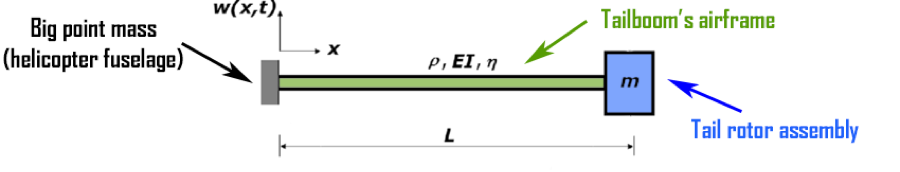
\includegraphics[width=0.95\linewidth]{PICTURES/2_Lama_truss/PNG/BC0.png}
	\end{center}
	%\caption{First approximation model of the tailboom}
\end{figure}	
%\vspace{0.5cm}


\clearpage
\subsection*{Full model's natural frequencies}
\noindent
Again, the first 10 resonant frequencies of the full model, obtained at the end of the convergence analysis, are displayed in the following results table:
\begin{figure}[h!]
	\begin{center}
		\centering  		 		
		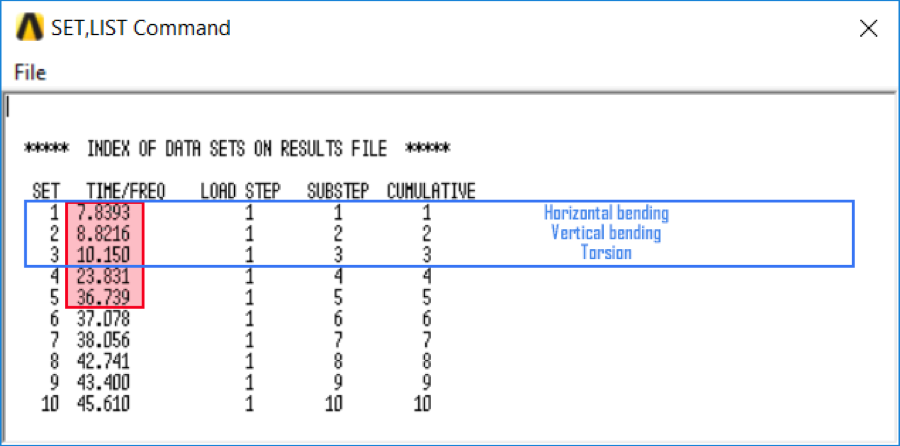
\includegraphics[width=0.70\linewidth]{PICTURES/2_Lama_truss/PNG/model2/set-list2.png}
	\end{center}
	\caption {List the first 10 computed natural frequencies computed}
\end{figure}
\noindent
As the case of the simple model, the first three regards the case of horizontal, vertical bending and torsion but they results to be lowered down. This fact match with our expectation since the \underline{subsystems} \underline{add weight and inertia to the whole structure shifting down its dynamical behaviour} toward lower frequencies.
Tu sum up, the following picture represents the results obtained for the simple and complete truss airframe models. 
\begin{figure}[h!]
	\begin{center}
		\centering  		 		
		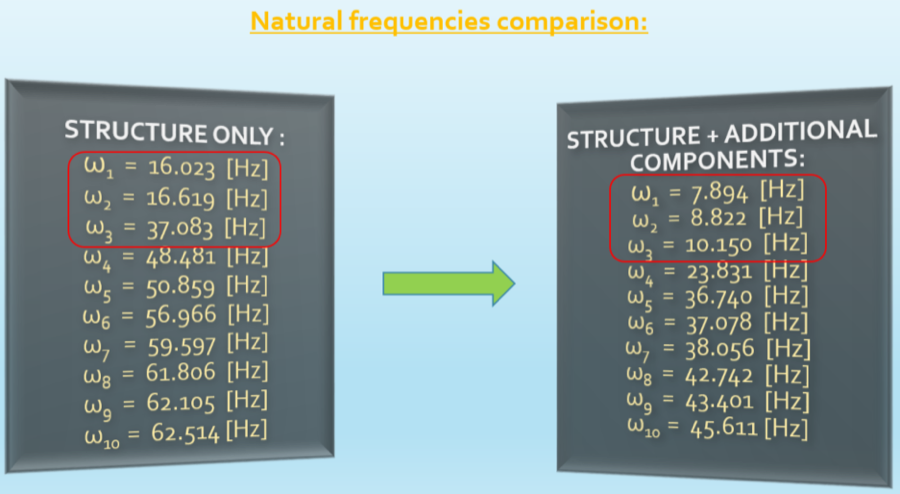
\includegraphics[width=0.70\linewidth]{PICTURES/2_Lama_truss/PNG/model2/comparison.png}
	\end{center}
	%\caption {List the first 10 computed natural frequencies computed}
\end{figure}

\smallskip
\noindent
IMPORTANT NOTE: \\
At this stage, those resonant frequencies are computed without considering the tail-rotor rotation. To consider the dynamic effects linked to the rotation of the system we must perform a \emph{tailrotor-fuselage coupled analysis}, as introduced in the chapter 4. \\ 






















\clearpage
\bigskip
	\chapter{Ecureuil AS-350 (semi-monocoque)}
\label{ch:Eurocopter AS350 (monocoque frame)}

\noindent
\emph{Another finite-element model regarding a modern semi-monocoque type of tailboom's design has been developed in order to compare and predict the vibration characteristics of the newer rotorcraft machines such as the Eurocopter AS-350 here presented.}

\section*{Introduction}
\addcontentsline{toc}{section}{Introduction}
\noindent
The \textbf{Eurocopter AS-350 Écureuil} is a single-engine light helicopter originally designed and manufactured in France by Aérospatiale, now Airbus Helicopters. It is widely spread for its unparalleled high-altitude capabilities and performance and has proven to be the most safe and reliable helicopter in the industry. \\
It has really close dimensions and technical specifications to the lama's helicopter and it is commonly considered its direct evolution. In fact, in the early 1970s, Aérospatiale decided to initiate a new development programme to produce a suitable replacement for the aging Aérospatiale Alouette II (Lama) for a new civil-orientated operations. \\
The development of the new rotorcraft, which was headed by Chief Engineer René Mouille, was focused on the production of an economic and cost-effective aerial vehicle, thus both Aérospatiale's Production and Procurement departments were heavily involved in the design process.
One such measure was the use of a rolled sheet structure, a manufacturing technique adapted from the automotive industry; another innovation was the newly developed Starflex main rotor. Right now, more than 3700 Ecureuil have been sold in the world overcoming millions of flying hours time.

\begin{figure}[t]
\centering
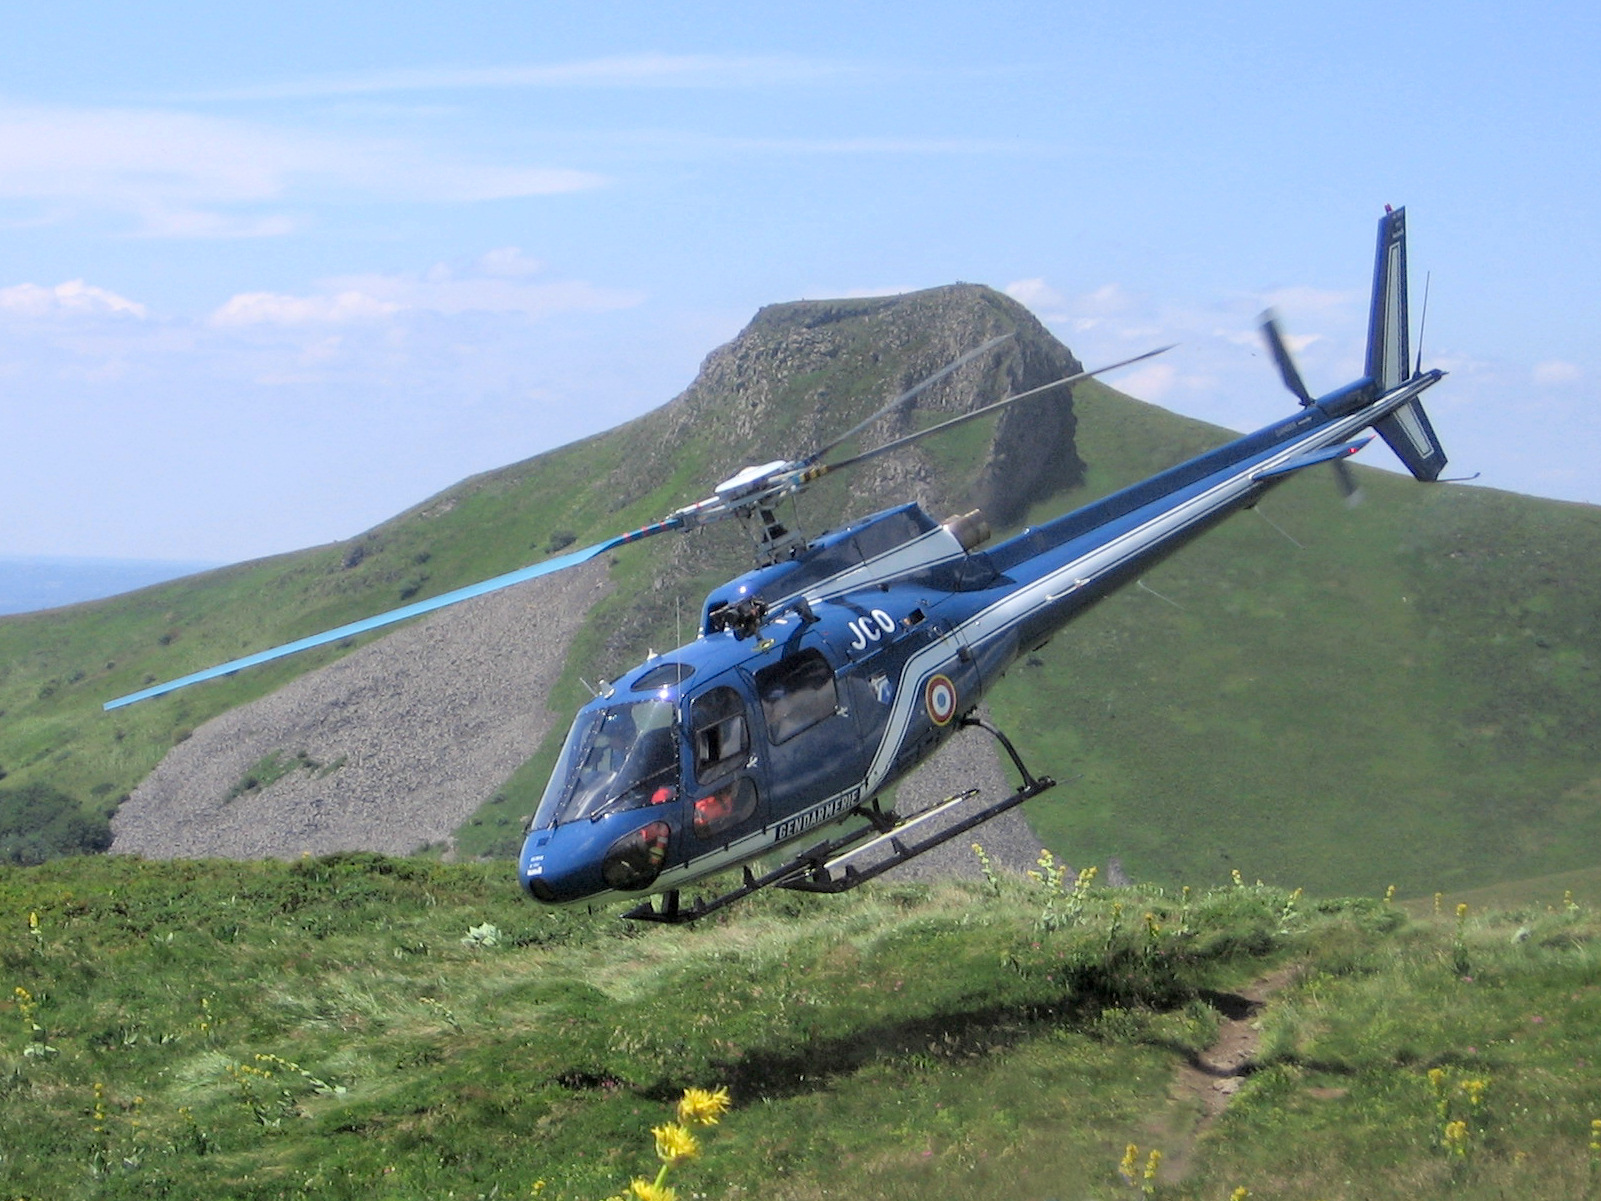
\includegraphics[width=0.80\textwidth]{imgs/Helicopter_rescue_sancy_takeoff}
\caption{Helicopter takeoff \\Di Fabien1309 - Own work}
\label{fig:AS350wiki}
\end{figure}

\begin{minipage}{\textwidth}
  \begin{minipage}[b]{0.49\textwidth}
   	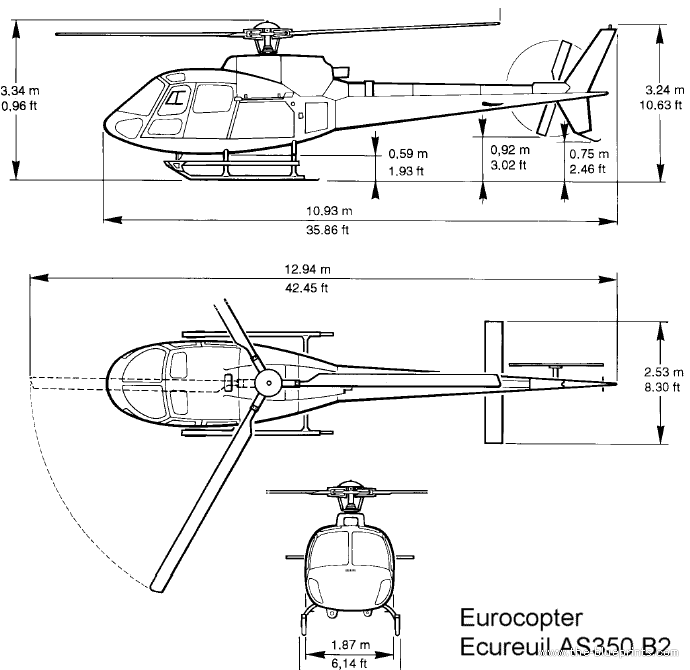
\includegraphics[width=\textwidth]{imgs/eurocopter-as350-b2}
    \captionof{figure}{AS350 blueprints\label{fig:AS350blueprints}}
  \end{minipage}
  \hfill
  \begin{minipage}[b]{0.49\textwidth}
    \centering
    \begin{tabular}{%
		>{}l%
		>{}l%
		>{\columncolor{yellow}}r}
		\multicolumn{2}{>{\columncolor{lightgray}}c}{General characteristics}\\
		Length	&	12.94 m\\
		Height	&	3.34 m\\
		Main rotor diameter& 10.69 m\\
		Empty weight		& 1220 kg\\
		Max takeoff weight & 2250 kg\\
		capability	& 2500 kg\\
		\multicolumn{2}{>{\columncolor{lightgray}}c}{Propulsion}\\
		Powerplant	&	1 x Turbine\\ 
		& Turbomeca\\& Arriel 1D1\\
		Power	&	546 kW\\
		\multicolumn{2}{>{\columncolor{lightgray}}c}{Performance}\\
		Maximum speed & 287 km/h\\
		Range	 & 476 km\\
		service ceiling 	 & 6100 m\\
    \end{tabular}
  \captionof{table}{Main characteristics AS350}\end{minipage}
\end{minipage}

\subsection*{General structural description}
\addcontentsline{toc}{subsection}{General structural description}
\noindent
The semimonocoque airframe, as introduced in chapter 1, is composed of:
\begin{itemize}
	\item longitudinal longerons;
	\item vertical formers and bulkhead; 	
	\item stringers;
	\item external skin.
\end{itemize}

\noindent
All these elements are designed to be attached together and to the skin to achieve the full strength benefits of semimonocoque design. It is important to recognize that the metal skin or covering carries
part of the load in this type of construction. \\
Furthermore, \emph{spreading loads among these structures and the skin means no single piece is failure critical and so, the fuselage may withstand considerable damage before failing}. \\

%\smallskip
\begin{figure}[h!]
	\begin{center}
		\centering  		 		
		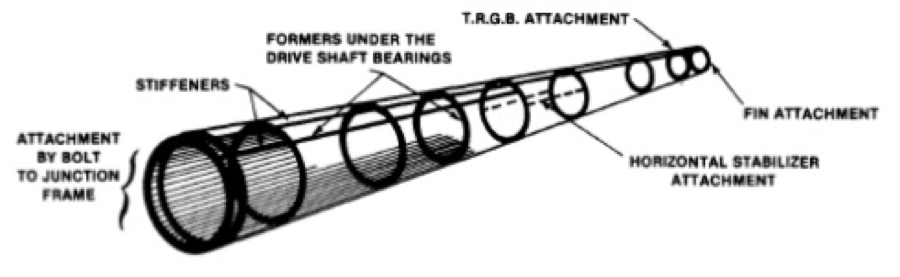
\includegraphics[width=0.9\linewidth]{PICTURES/3_Ecureuil/semimonocoque2}
	\end{center}
	\caption{Elements in a semimonocoque construction}
\end{figure}	
%\vspace{0.5cm}



\section*{Material properties}
\addcontentsline{toc}{subsection}{Material properties}
\noindent
The semimonocoque fuselage is constructed primarily of alloys of aluminum, although steel is adopted for the formers that support the drive shaft bearings and for the junction frame, attached by bolts, to the cockpit.

\begin{table}[h!]
	\centering
	
	\begin{tabular}{c c c c} 
		\toprule
		\multicolumn{4}{c}{Material properties}\\
		\midrule
		Mat & Density (kg/m3) & Poisson's ratio & Young's modulus (GPa) \\
		\midrule
		Steel & 7850  &  0.29 & 205 \\ 
		\midrule
		Aluminium & 2700  &  0.34 & 64 \\
		\bottomrule
	\end{tabular}	
\end{table}

\clearpage
\section*{Element types}
\addcontentsline{toc}{subsection}{Element types}
\noindent
The semimonocoque's model has been discretized using the following element's types:
\begin{itemize}
	\item \textbf{BEAM 189}: with rectangular cross-section to model Longerons and stringers, as shown in \ref{subfig:Rectagnle}, and with square cross-section to model stiffners \ref{fig:SectionGeometry};
	\item \textbf{SHELL 181}: to model the outer aluminium skin which compose the coverage of the structure;
	\item \textbf{MPC 184}: to rigidly connect to the airframe the concentrated masses representing the tail rotor drive shaft supported by its bearings.
\end{itemize}
%
The complete structure skeleton is represented in fig. \ref{fig:Skeleton}.
%
\bigskip
\begin{table}[h!]
	\centering
	
	\begin{tabular}{c c r l} 
		\toprule
		\multicolumn{4}{c}{Tubes cross section's properties}\\
		\midrule
		Family & Parameter & Value & Description \\
				
		\midrule
		& $length$ &  5.2 $[m]$ & Total tail length \\
		& $b \, * \, h$ &  9 x 1.5 $[mm]$ &  Cross section's dimensions\\ 
		Longerons & $A_{section}$  &  13.5 $[mm^2]$ & Area of the cross section \\ 
		& $I_{x} = I_{y}$ &  $91.125$ $[mm^4]$ & Moment of inertia \\ 
		
		
		\midrule
		& $length$ &  5.2 $[m]$ & Total length \\
		& $b \, * \, h$ &  5 * 5 $[mm]$ &  Cross section's dimensions\\ 
		Stiffners & $A_{section}$  &  25 $[mm^2]$ & Area of the cross section \\ 
		& $I_{x} = I_{y}$ &  $52.08$ $[mm^4]$ & Moment of inertia \\ 	
		
		\bottomrule
	\end{tabular}
	\caption{Structural elements characteristics}
	
\end{table}

\begin{figure}[!htb]
	\centering
	\subfloat[][\emph{Rectangular}.\label{subfig:Rectagnle}]{
		\resizebox{.25\linewidth}{!}{\begin{tikzpicture}
%linee guida
%\foreach \x in {0,1,...,15}
%   \draw [help lines] (\x,0) node [below,%
%          font=\footnotesize] {$\x$} -- (\x,15);
%%\foreach \y in {0,1,...,15}
%%   \draw [help lines] (0,\y) node [left,%
%%          font=\footnotesize] {$\y$} -- (15,\y);

\node at (1,14) (a) {};
\node at (3,14) (b) {};
\node at (3,10) (c) {};
\node at (1,10) (d) {};

\draw (a) rectangle (c);
\draw[-latex] (2,12)--( 2,9.5)node[right]{\scriptsize x};
\draw[-latex] (2,12)--(3.5,12)node[above]{\scriptsize y};


% quote track
 \dimline    [color=gray,
 			  label style={above=0.1ex},
                % line style={thick},
                %extension start style={gray,thin},
                %extension end style={gray,thin},
                extension start length=0.5cm,
                extension end length=0.5cm
                ]{(1,14.5)}{(3,14.5)}{$b$};
                
\dimline    [color=gray,
                % line style={thick},
                %extension start style={gray,thin},
                %extension end style={gray,thin},
                extension start length=0.5cm,
                extension end length=0.5cm
                ]{(0.5,10)}{(0.5,14)}{$w$};
\end{tikzpicture}}} \quad
	\subfloat[][\emph{Square}.\label{subfig:Square}]{
		\resizebox{.25\linewidth}{!}{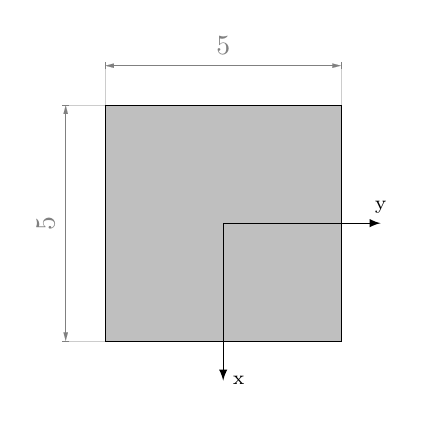
\begin{tikzpicture}
%linee guida
%\foreach \x in {0,1,...,15}
%   \draw [help lines] (\x,0) node [below,%
%          font=\footnotesize] {$\x$} -- (\x,15);
%\foreach \y in {0,1,...,15}
%   \draw [help lines] (0,\y) node [left,%
%          font=\footnotesize] {$\y$} -- (15,\y);

\node at (1,14) (a) {};
\node at (4,14) (b) {};
\node at (4,11) (c) {};
\node at (1,11) (d) {};

\draw[fill=lightgray] (a) rectangle (c);
\draw[-latex] (2.5,12.5)--( 2.5,10.5)node[right]{\scriptsize x};
\draw[-latex] (2.5,12.5)--(4.5,12.5)node[above]{\scriptsize y};


% quote track
 \dimline    [color=gray,
 			  label style={above=0.1ex},
                % line style={thick},
                %extension start style={gray,thin},
                %extension end style={gray,thin},
                extension start length=0.5cm,
                extension end length=0.5cm
                ]{(1,14.5)}{(4,14.5)}{$5$};
                
\dimline    [color=gray,
			label style={above=0.1ex},
                % line style={thick},
                %extension start style={gray,thin},
                %extension end style={gray,thin},
                extension start length=0.5cm,
                extension end length=0.5cm
                ]{(0.5,11)}{(0.5,14)}{$5$};
\end{tikzpicture}}}\\
	\caption{Section for element \textsc{beam189}}
	\label{fig:SectionGeometry}
\end{figure}

\clearpage
\section*{Approach to the problem}
\section{Geometric model (airframe only)}
\subsection*{Analysis model}
\addcontentsline{toc}{subsection}{Analysis model}

\noindent
We approached this problem with the same steps of the previous helicopter's tail model. Firstly only the naked airframe has been studied considering it just as a cantilever beam, then, subsystems have been added to increase the accuracy of the model adding the drive shaft (considered as distributed masses along the tail's length) and other concentrated masses and inertias to represent the tail rotor assembly at the tail's tip. \\

\noindent
The created model can be seen in the figure \ref{fig:AnsysMeshLump}.

\medskip
\begin{figure}[h!]
	\begin{center}
		\centering  		 		
		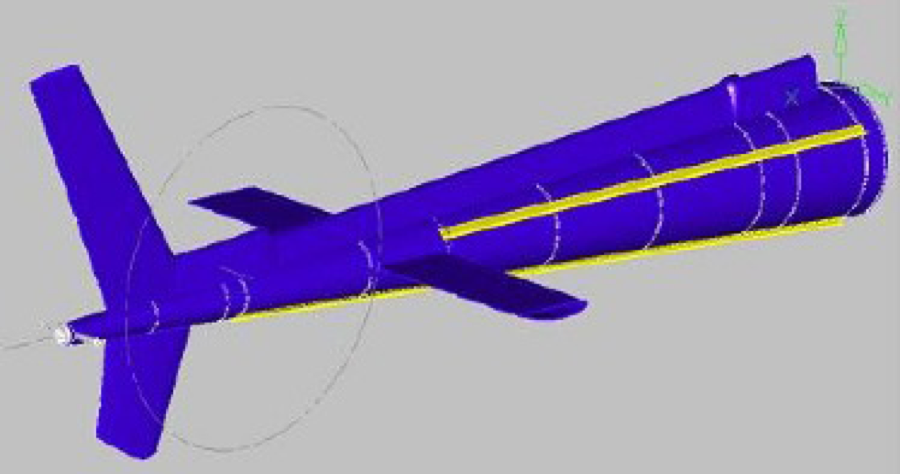
\includegraphics[width=0.8\linewidth]{PICTURES/3_Ecureuil/analysis_model}
	\end{center}
	\caption{Analysis model}
\end{figure}	
%\vspace{0.5cm}

\medskip
\begin{table}[h!]
	\centering
	
	\begin{tabular}{c c r l} 
		\toprule
		\multicolumn{4}{c}{Tubes cross section's properties}\\
		\midrule
		Family & Parameter & Value & Description \\
		\midrule
		& base radius &  \textbf{325} $[mm]$ & Base radius (cone) \\
		& top radius &  \textbf{50} $[mm]$ & Top radius (cone) \\
		Model dimensions & tail length &  \textbf{5.2} $[m]$ & Total tail length \\
		& 7 segments &  \textbf{0.74} $[m]$ & Total segment length \\
		& skin thickness &  $\textbf{0.5}$ $[mm]$ & Shell thickness \\
		\bottomrule
	\end{tabular}
	\caption{Tailboom's model dimensions}
	
\end{table}


\clearpage
\subsection*{Model assumptions}
\addcontentsline{toc}{subsection}{Model assumptions}

\noindent
\begin{quoting}
	\begin{itemize}
		
		\item Element type: \textbf{BEAM 189} based on Timoshenko beam theory which includes shear-deformation effects and \textbf{SHELL 181} elements to discretize the structure;
		
		\item uniform cross-sections of the elements and of the shell thickness along the tail's length;
		
		\item riveting and bolting connections of the coverage skin not considered;
		
		\item \underline{linear elastic isotropic} material properties;
		
		\item self-weight of the elements considered;
		
		\item geometrical non-linearities included in the static analysis (NLGEOM,ON) \\
		
	\end{itemize}
\end{quoting}

\smallskip
\subsection*{Tailboom geometric model (airframe only)}

\begin{figure}[!htb]
	\centering
	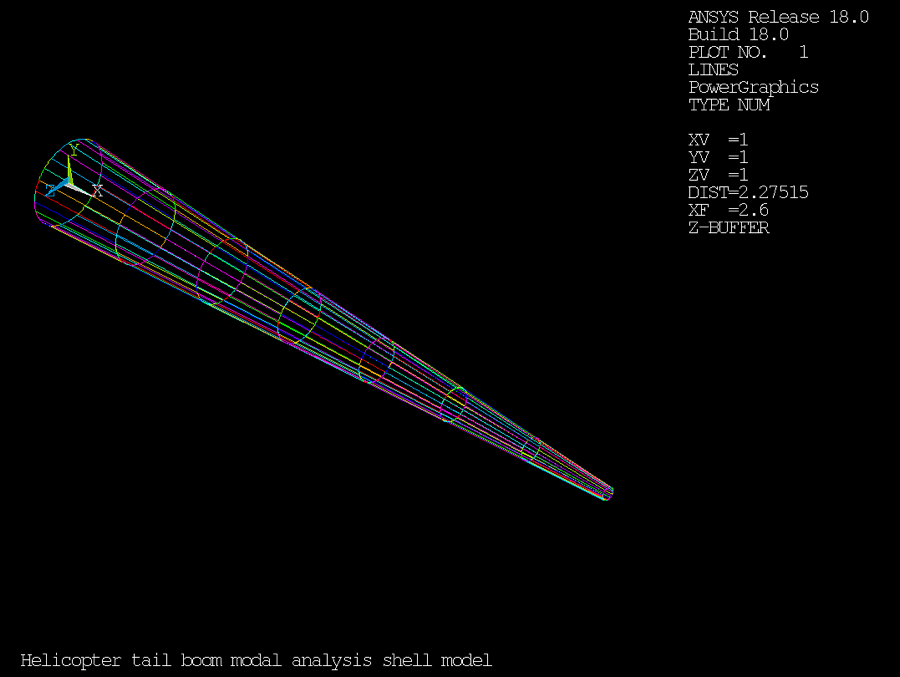
\includegraphics[width=0.75\textwidth]{PICTURES/imgs/ShellModel/img/Shellmodel000.png}
	\caption{Model geometry (isometric view)}
	\label{fig:Geometric}
\end{figure}


\begin{figure}[!htb]
	\centering
	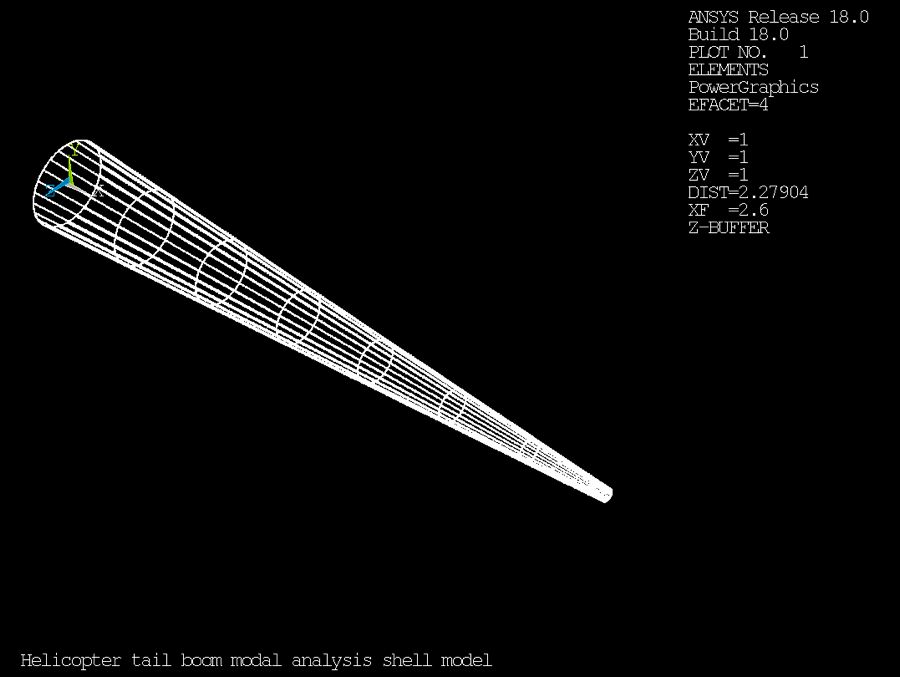
\includegraphics[width=0.75\textwidth]{PICTURES/imgs/ShellModel/img/Shellmodel001.png}
	\caption{Tailbooms skeleton (isometric view)}
	\label{fig:Skeleton}
\end{figure}



\subsection*{Aluminium's outer skin}
\noindent
The outer skin which represents the external coverage of the airframe and which contributes to support part of the external load has been modelled using SHELL 181 elements of constant thickness. 
Riveting connections have not been modelled for simplicity.
%
\begin{figure}[!h]
	\centering
	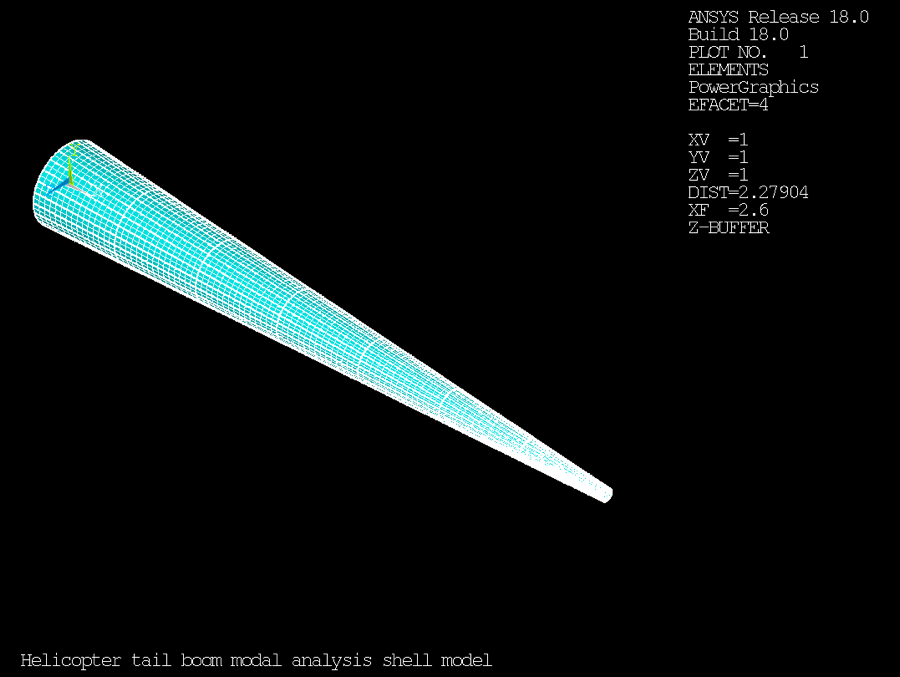
\includegraphics[width=0.75\textwidth]{PICTURES/imgs/ShellModel/img/Shellmodel002.png}
	\caption{Aluminium's outer skin}
	\label{fig:AnsysMeshLump}
\end{figure}
%
\subsection*{Applied loads and boundary conditions}
\addcontentsline{toc}{subsection}{Applied loads and boundary conditions}
\noindent
The loads considered for the static analysis are exactly the same of the previous model, but the force is applied at the rotor hub's attaching point which, in this case, is not at the tail tip but at a point near the rear end. \\
For the boundary conditions, again the tail is considered as a cantilever beam but this time the all nodes of the base junction have been constrained to the ground. \\


\section{Preliminary static analysis}
\noindent
As we saw before, the preliminary static analysis is performed in such a way to check if the all structure is well posed and ready for the modal analysis.
So, we have looked into the deformation caused by the self-weight of the structure, due to the gravity acceleration, and to the tail rotor thrust force. 



\subsubsection*{PLDISP and PLNSOL (node's displacement)}
%\smallskip
\begin{figure}[h!]
	\begin{center}
		\centering  		 		
		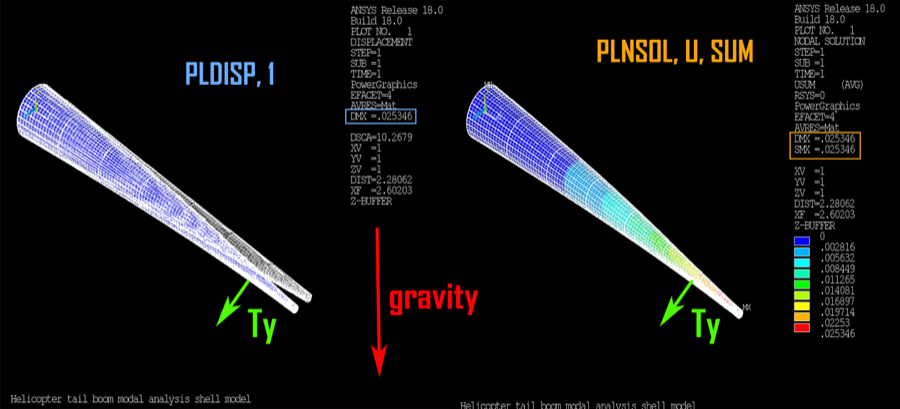
\includegraphics[width=0.95\linewidth]{PICTURES/3_Ecureuil/static_analysis_simple.png}
	\end{center}
	%\caption{Model's boundary conditions}
\end{figure}	
%\vspace{0.5cm}

\noindent As a matter of fact, we can observe that this value (maximum displacement) 
compared among both models is very closed each other. We can also prove that shell model is more flexible than the truss model, as a consequence of a bigger total displacement.\\
Furthermore it is evident that in the normal operation the tailboom is \textbf{pre-loaded} by the aerodynamic thrust force provided by the tailrotor. This pre-load as an effect on the vibrational behaviour of the system. 



\clearpage
\section*{Modal Analysis (airframe only)}
\addcontentsline{toc}{subsection}{Modal Analysis (airframe only)}
\noindent
After a mesh refinement and a convergence analysis, the first 20 values of the natural frequencies of the shell monocoque airframe have been extracted and are now listed in the following table:

\begin{table}[h!]
	\centering
	\pgfplotstableset{
		% global config, for example in the preamble
		% these columns/<colname>/.style={<options>} things define a style
		% which applies to <colname> only.
		every head row/.style={before row=\hline,after row=\hline},
		every last row/.style={after row=\hline},
		display columns/0/.style={column name =Mode, int detect,column type=r},
		display columns/1/.style={column name =Frequence [Hz], column type=r,
			fixed,fixed zerofill,precision=5,set thousands separator={\,}},
		%other style option   
	}
	\pgfplotstabletypeset[col sep=space]{ModalFreq-Shellmodel.txt}
	\caption{Natural frequencies for the simple model}
	\label{tab:ModalFreq-Shellmodel}
\end{table}


\bigskip
\noindent
IMPORTANT NOTE: \\
The applied boundary conditions (fixed - free) constrain the structure in order to be \textbf{statically determinate}. In fact, NO zero-frequency modes have been found, as it can be seen in the table 3.4.
So, the stiffness matrix of our structure, thanks to the type of the constraint, results to be \textbf{positive definite} and NO rigid motions of the system occur. \\




\clearpage
\section{Full shell model (airframe + subsystems)}

\noindent
Starting from the simple airframe model, concentrated masses with rigid links are added to represent the aircraft subsystems in a lumped formulation. \\ The element used is the well known \textsc{mass21} with mass and inertia concentrated properties. This introduce an approximation in the analysis of the structure but it allows it to be simpler and computationally lighter to be solved. \\
In the following picture, the components we intend to model are shown on a real Ecureil helicopter type: \\ 


\begin{figure}[h!]
	\begin{center}
		\centering  		 		
		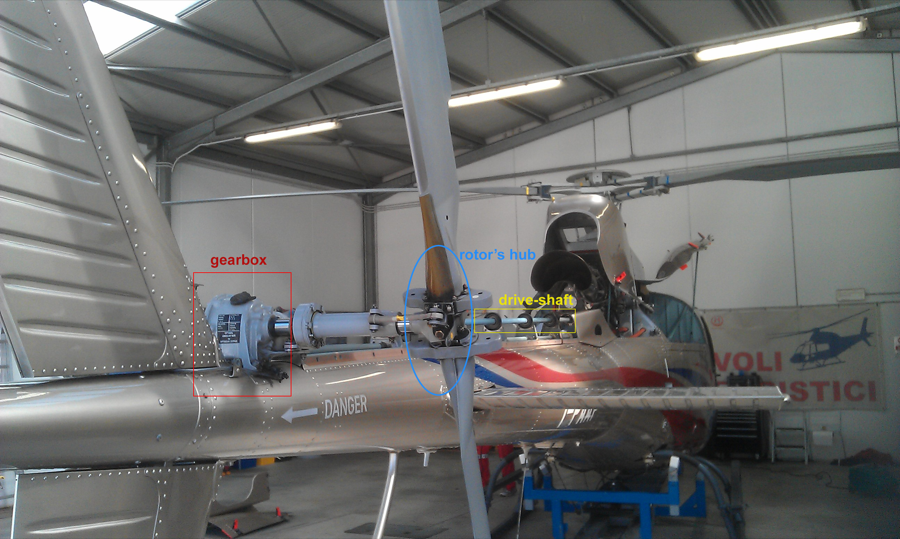
\includegraphics[width=1\linewidth]{PICTURES/3_Ecureuil/IMAG0112.png}
	\end{center}
	\caption{Drive-shaft, gearbox and rotor assembly parts}
\end{figure}	
\vspace{0.5cm}


\noindent
In order to ensure rigid connections between the concentrated masses and the airframe structure, elements of type: \textsc{mpc184}, with key option: $1$, are used to block six degrees of freedom for each element. \\

\noindent
The gearbox is attached in the rear three-quarter of the tailboom and considered again as a lumped mass by using the element type \textsc{mass21} located on the last bearing node. \\

\clearpage
\medskip
\noindent
The following list contains the values of the concentrated masses considered in the model:

\begin{itemize}
	\item drive shaft total mass: $12\,[kg]$ divided on the 7 support bearings along the tail;
	\item gearbox concentrated mass: $30\,[kg];$
	\item rotor assembly: $15\,[kg];$
\end{itemize}

\medskip
\begin{figure}[h!]
	\begin{center}
		\centering  		 		
		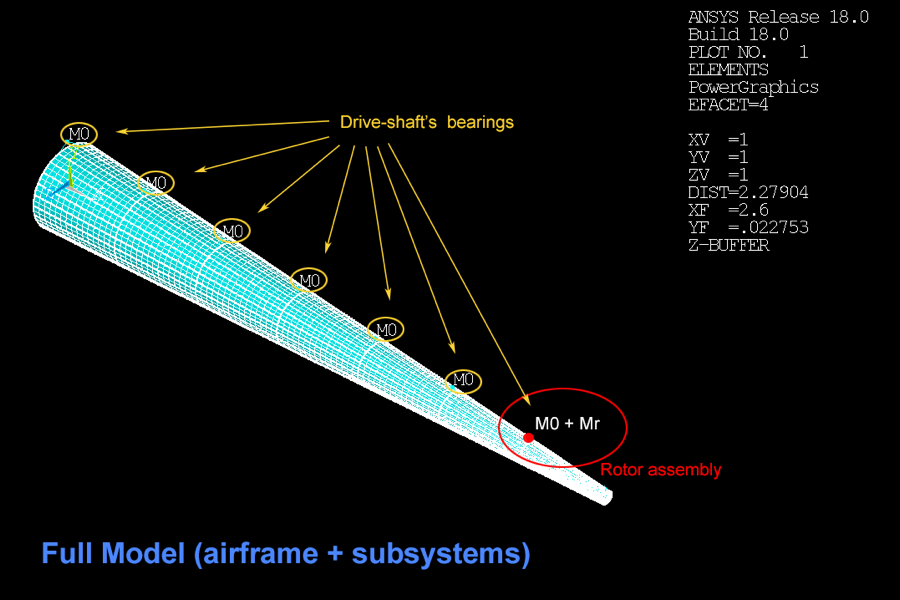
\includegraphics[width=0.95\linewidth]{PICTURES/3_Ecureuil/full_model.png}
	\end{center}
	\caption{Complete shell model ready for the modal analysis.}
\end{figure}	
\vspace{0.5cm}




\clearpage
\section*{Modal Analysis (full tail model)}
\addcontentsline{toc}{subsection}{Modal Analysis (full tail model)}
\noindent

\noindent
After a mesh refinement and a convergence analysis, the first 20 values of the natural frequencies of the shell semi-monocoque airframe have been extracted and are now listed in the following table \ref{ModalFreq-ShellmodelShaftLumped}:

\begin{table}[!h]
	\centering
	\pgfplotstableset{
		% global config, for example in the preamble
		% these columns/<colname>/.style={<options>} things define a style
		% which applies to <colname> only.
		every head row/.style={before row=\hline,after row=\hline},
		every last row/.style={after row=\hline},
		display columns/0/.style={column name =Mode, int detect,column type=r},
		display columns/1/.style={column name =Frequence [Hz], column type=r,
			fixed,fixed zerofill,precision=5,set thousands separator={\,}},
		%other style option   
	}
	\pgfplotstabletypeset[col sep=space]{ModalFreq-ShellmodelShaftLumped.txt}
	\caption{Natural frequencies for the model with lumped mass}
	\label{ModalFreq-ShellmodelShaftLumped}
\end{table}%

\bigskip
\noindent
IMPORTANT NOTE: \\
\noindent
As before, those resonant frequencies are computed without considering the tail-rotor rotation.
The \emph{tailrotor-fuselage coupling} will be introduced in the next chapter.

\clearpage

\subsection*{Modal shapes}
\noindent
Eigenvectors are typically normalized in Ansys with respect to the mass matrix and; this normalization is very useful from the computational point of view. However, the drawback is that in this way they represent correctly the shape of the mode but not the real amplitude of the displacement which in turn depends on the initial conditions. 

\begin{figure}[h]
	\begin{center}
		\centering  		 		
		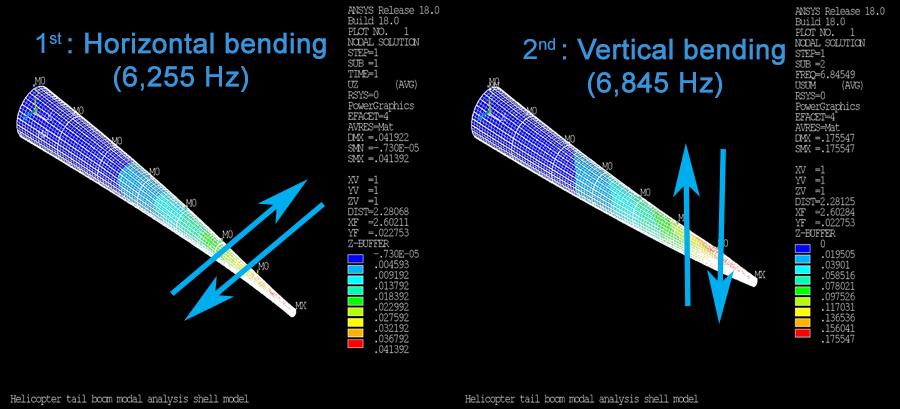
\includegraphics[width=0.95\linewidth]{PICTURES/3_Ecureuil/1-2.png}
	\end{center}
	\caption {Graphical representation of the first and second modal shapes}
\end{figure}

\noindent
The first three mode shapes are related to the \emph{horizontal,vertical and torsional} movement of the tailboom. The last one shows the shell expansion effect. 

\begin{figure}[h]
	\begin{center}
		\centering  		 		
		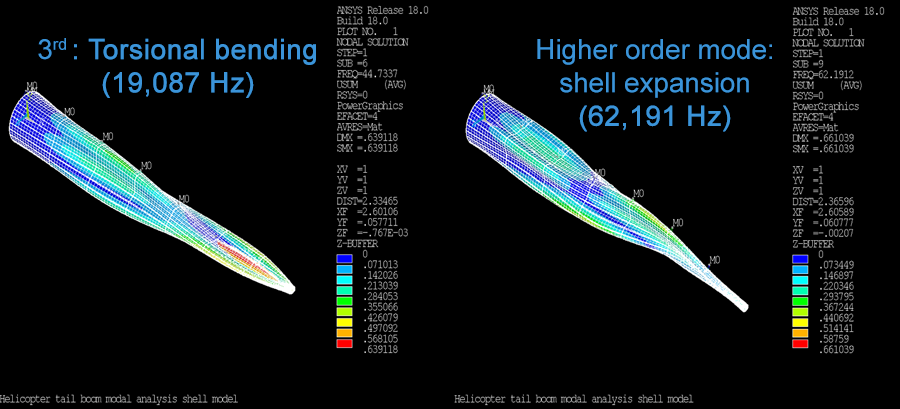
\includegraphics[width=0.95\linewidth]{PICTURES/3_Ecureuil/3-4.png}
	\end{center}
	\caption {Graphical representation of higher order modal shapes}
\end{figure}

	\chapter{Rotor-fuselage dynamic coupling}
\label{ch:Rotor-fuselage dynamic coupling}

\subsection*{Rotating systems}
\addcontentsline{toc}{subsection}{Rotating systems}
\noindent
\underline{The rotation of the tail-rotor}, which is obviously spinning during the flight condition, \underline{considerably affect the vibrational behaviour of the tailboom} with respect to the case in which the rotor is still (for example on the ground with engine off). \\
In rotating systems, in fact, the dynamic behaviour undergoes considerable variations due to the fenomena related to the rotation of the systems, which are basically:
\begin{itemize}
	\item the onset of \textbf{gyroscopic moments}, function of the angular velocity $\Omega$;
	\item the presence of \textbf{static} or \textbf{dynamic} unbalances which produces excitations also function of $\Omega$. 
\end{itemize}

\noindent
The consequence of those phenomena is that the whole system, at each angular velocity, has natural frequencies different from those relative to the system in rest and those frequencies results also variable with $\Omega$. \\
\noindent
Furthermore, when the rotor system is fixed on the tailboom, the two systems dynamically interact to each other and those effects must be taken into account in order to accurately model the real system's dynamic behaviour. \\

\noindent
In the literature, there have been many attempts to predict the vibration of a rotor-body coupled system with a variety of assumptions and solution methods; anyway, from most of those past studies \underline{there appears to be no viable alternative to carrying out a coupled} \underline{rotor-fuselage analysis when one is investigating fuselage response to rotor excitation}, in order to represent accurately the real system's behaviour. \\

\noindent
So, 3 possible ways to treat the coupling will be presented in the next section which is only intended as possible hints to extend this project for further improvements.  


\clearpage
\section*{Hints on possible approaches}
\addcontentsline{toc}{subsection}{Hints on possible approaches}
\noindent
The fuselage's equations of motion and the rotor's ones results to be coupled. \\
There are different possible approaches to solve a coupled problem:

\medskip
\subsubsection*{a) Complete Coupled Formulation}
\addcontentsline{toc}{subsubsection}{a) Complete Coupled Formulation}
\noindent
In this case, all the linear terms of the rotor and fuselage equations are transferred from the right hand side to the left hand side of the equation.

\smallskip
\begin{figure}[h]
	\begin{center}
		\centering  		 		
		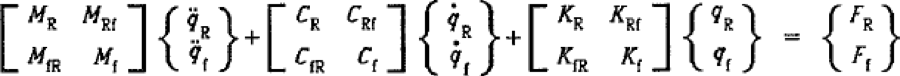
\includegraphics[width=0.9\linewidth]{PICTURES/3b_coupling/eq_1.png}
	\end{center}
	\caption {Complete coupled formulation equations}
\end{figure}
%\vspace{0.5cm}


\underline{Advantage}: 
\begin{itemize}
	\item Direct evaluation of the eigenvalues and eigenvectors of the system;
\end{itemize}



\underline{Disadvantages}: 
\begin{itemize}
	\item Inflexibility of changing any of the terms;
	\item It require linearization of the force terms which lead to additional assumptions and approximations.
\end{itemize}

\medskip
\subsubsection*{b) Explicit Coupled Formulation}
\addcontentsline{toc}{subsubsection}{b) Explicit Coupled Formulation}
\noindent
This second approach is based on an advanced technique for solving non-linear sets of equations. The rotor/body coupled system of equations are formulated in the following explicit form:

\smallskip
\begin{figure}[h]
	\begin{center}
		\centering  		 		
		\includegraphics[width=0.9\linewidth]{PICTURES/3b_coupling/eq_2.png}
	\end{center}
	\caption {Explicit coupled formulation equations}
\end{figure}
%\vspace{0.5cm}

\noindent
Here the rotor/fuselage coupling terms lie on the right hand side with external forces. Therefore the right hand terms are function of the rotor as well as fuselage motion. Rotor and fuselage equations are solved iteratively. The converged solution represents a fully coupled system.

\medskip
\underline{Advantages}: 
\begin{itemize}
	\item Flexibility in changing the fuselage modelling;
	\item It is possible to identify the coupling terms in the forcing expression.
\end{itemize}

\underline{Disadvantage}: 
\begin{itemize}
	\item direct evaluation of the coupled system eigenvalues and eigenvectors has to be done only by frequency sweep;
	\item requires a non-linear solver
\end{itemize}


\bigskip
\subsubsection*{c) Simulate gyroscopic effects with rotational springs}
\addcontentsline{toc}{subsubsection}{c) Simulate gyroscopic effects with rotational springs}
\noindent
This third case, consists in simplifying the problem considering the rotor as a concentrated mass and inertia and introducing \underline{rotational springs} that act on the fuselage for modeling the gyroscopic effects that appears when moments or forces act on the spinning rotor making it rotate around on of its axes. 

\medskip
\underline{Disadvantages}: 
\begin{itemize}
	\item It is an approximation; even introducing an equivalent rotor mass, although it gives a somewhat
	better approximation, still does not adequately represent the coupled rotor-fuselage system;
	\item Rotational springs musts apply a moment in a plane orthogonal to the one in which the rotation occours (difficult to implement);
	\item Stiffness properties of the springs are not constant  (vary with the rotor's speed $\Omega$).
\end{itemize}


\bigskip
\noindent
The first two methods have been taken from literature from a NASA research article (cited in the bibliography) while the third method is just a proposal in order to simplify and treat this complex problem in a easier way. \\
Many other methods can be found in literature to solve this particular problem and each of them has different assumptions and limitations. The choice in one of them depends on project's purposes and expectations.


\clearpage
\subsection*{Effect of the rotor-fuselage dynamic coupling on the system's natural frequencies}
\addcontentsline{toc}{subsection}{Effect of the rotor-fuselage coupling}
\noindent
In the following pictures, taken from the literature, it is outlined the effect of the rotor-fuselage dynamic coupling on the system's resonant frequencies. \\
It is is clear that the dynamic coupling cannot be neglected if an accurate model is needed. In fact, it is evident that system's natural frequencies significantly change with rotor's speed and at each speed they are different from the frequencies at still condition. \\

\smallskip
\begin{figure}[h]
	\begin{center}
		\centering  		 		
		\includegraphics[width=0.85\linewidth]{PICTURES/3b_coupling/1.png}
	\end{center}
	\caption {Coupled and uncoupled rotor-fuselage eigenvalues}
\end{figure}

	\chapter{Rotor-dynamic analysis}


\noindent
From this point onwards, the tail-rotor behaviour has been investigated implementing a simplified FEM model and taking advantage of the Rotordynamics capabilities of Ansys. \\
From the definition of ANSYS help, \textit{Rotor-dynamics is the study of vibrational behaviour in axially symmetric rotating structures}. At high rotational speeds, such as in a helicopter's tail rotor, the inertia effects of the rotating parts must be consistently represented in order to accurately predict the rotor behaviour. An important part of the inertia effects is the \underline{gyroscopic moment} introduced by the precession motion of the rotor which is function of the spin velocity. Hence, the velocity term in the equation of motion as well as the support flexibility and damping behaviour cannot be neglected and they are important factors in enhancing the stability of the vibrating rotor.



\section*{Modal analysis of rotating structures}
\addcontentsline{toc}{section}{Modal analysis of rotating structures}
\noindent
The modal analysis allows for the calculation of natural frequencies and critical speeds (Campbell diagram) of the rotor. \\
From dynamical point of view, the equations of motion of a generic rotating structure is:
\medskip

\begin{equation*}
\left[ M \right] \left\lbrace \ddot{u} \right\rbrace + \left( \left[ C \right] + \left[ G \right] \right) \left\lbrace \dot{u} \right\rbrace + \left( \left[ K \right] - \left[ K_c \right] \right) \left\lbrace u \right\rbrace = \left\lbrace 0 \right\rbrace
\end{equation*}


\medskip
\noindent
where [G] is the gyroscopic matrix that depends on the rotational velocity and is the major contributor to tailboom's rotor, while [$K_c$], the spin softnening matrix, also depends upon the rotational velocity and it modifies the apparent stiffness of the structure. \\
This equation holds when motion is described in a stationary reference frame.

\clearpage
\noindent
\underline{STEPS FOR MODAL ANALYSIS IN ANSYS}: \\
\begin{itemize}
	\item 1) Model implementation; 
	
	\item 2) Boundary conditions; 
	
	\item 3) Solution including rotational effects (centrifugal and Coriolis); 
	
	\item 4) Postprocessing. \\
\end{itemize}



\subsection*{Tail rotor simplified model}
\addcontentsline{toc}{subsection}{Tail rotor simplified model}
\noindent
A simplified model of the tail rotor has been defined, and built up in apart macro. It consists in the following parts:
\begin{itemize}
	\item \textbf{SHAFT}: elastically supported shaft modelled with BEAM 188 elements;
	\item \textbf{ROTOR'S HUB}: modelled with a lumped mass and inertia concentrated in the center of the rotor attached to a master node;
	\item \textbf{ROTOR}: modelled with a circular ring of SHELL 181 elements with radius passing through to the center of mass of the blades. CERIG elements have been introduced in order to connect the master node (hub) to the slave nodes of the ring.
\end{itemize}

\medskip
\begin{figure}[h]	
	\centering
	\subfloat[][\emph{real tail rotor assembly}.]
	{\includegraphics[width=.45\textwidth]{PICTURES/2_Lama_truss/PNG/model2/hqdefault2}} \quad
	\subfloat[][\emph{analysis model}.]
	{\includegraphics[width=.45\textwidth]{PICTURES/5_Rotordynamics/scheme.png}}\\
	\caption{Schemes of tail rotor assembly's model}
\end{figure}
%\vspace{0.5cm}

\subsection*{Model assumptions}
\addcontentsline{toc}{subsection}{Model assumptions}
\begin{itemize}
	\item Axial-symmetric structure (rotor-dynamics requirement in Ansys);
	\item Linear elastic material properties;
	\item Rotor elastically supported (2 bearings);
	\item Aerodynamic loads not considered;
	\item Rigid rotor and connections (no hinges or flexible joints).
\end{itemize}



\subsection*{Applied boundary conditions}
\addcontentsline{toc}{subsection}{Applied boundary conditions}
\noindent
\begin{itemize}
	\item Only fixed constraints are allowed for rotor-dynamic analysis;
	\item Support elasticity modelled using COMBIN14 elements to represent bearings;
\end{itemize}

\noindent
\textbf{COMBIN14} \\
Bearings have been modelled with COMBIN14 element whose properties simulate the effect of a longitudinal spring-damper as a axial tension-compression element.
The element is created between two nodes which, in our case, are overlapped. One of the nodes is rigidly attached to the shaft while the other one is constrained on the ground. These elements allows the elastic movement of the shaft in the Y and Z directions. The bearing is composed by 7 balls that ensure an overall stiffness equal to $378e+7$ N/m.\\

\medskip
\begin{figure}[h]
	\begin{center}
		\centering  		 		
		\includegraphics[width=0.55\linewidth]{PICTURES/5_Rotordynamics/2.png}
	\end{center}
	\caption {Tail rotor simplified model}
\end{figure}
%\vspace{0.5cm}

\clearpage
\subsection*{Solution including rotational effects (centrifugal and Coriolis)}
\addcontentsline{toc}{subsection}{Solution including rotational effects (centrifugal and Coriolis)}
\noindent
The modal analysis must be solved using an algorithm for damped modal analysis (complex Eigenvalues and Eigenvectors). We have chosen the \textbf{QRDAMP} solver including the rotational effects (\textbf{CORIOLIS, ON, , , ON}), as reported in listing (\ref{list:SolutionChunk}). The rotation speed (2000 RPM) has been divided in several load-steps. 10 modes have been extracted from each step. 

\lstinputlisting[firstline=133, lastline=146, language=apdl-modified,label={list:SolutionChunk}, caption=solution including rotational effects]{./COMMAND_LISTS/SOLO_ROTOR.txt}

\subsection*{Postprocessing}
\addcontentsline{toc}{subsection}{Postprocessing}
\noindent
Rotor's natural frequencies have been calculated for each value of the rotation speed (hence for each load step) and assigned to a substep. Resulting natural frequencies vary with the rotor speed as it is displayed in the campbell diagram below. \\
A \textbf{critical speed} appears when the natural frequency is equal to the excitation frequency, and excitation may come from unbalance that is synchronous with the rotational velocity. \\
Critical speeds are directly determined by solving a new eigenvalue problem or by performing a Campbell diagram analysis, where the intersection points between the frequency curves and the excitation line are calculated.

\noindent
The rotational velocity of the rotor is specified via the \textbf{CMOMEGA} command which requires to specify which is the rotating component, previously defined and selected as input for the velocity vector (magnitude and direction). \\
Then, we can set the \textbf{CAMPBELL, ON} Ansys' command. \\

\noindent
\textbf{NOTE:} \\
Bearing stiffness has an important effect on the critical speeds. When analysing a rotor, it is important to understand the effect of the bearing stiffness on the critical speeds and this can be done drawing the "Critical Speed Map" (here neglected).

\vspace{5mm}
\noindent
The rotor has been achieved with some parameters determined after performed a static analysis on ANSYS. The resulting given matrix provide us the information needed for establish some following conclusions:

\begin{equation*}
\left[ I \right] = \begin{bmatrix} 8.6440 & 0.1476 \times 10^{-3} & -0.3815 \times 10^{-4} \\ 0.1476 \times 10^{-3} & 14.487 & -0.1114 \times 10^{-3} \\ -0.3815 \times 10^{-4} & -0.1114 \times 10^{-3} & 13.895
\end{bmatrix} \quad
\end{equation*}

\vspace{3mm}
\noindent
As can be seen from the preceding matrix [\textit{I}], the diagonal guys refers to polar ($I_{p1}$ = 8.6440 $kg*m^2$) and diametrical inertia ($I_{d2}$ = 14.487 $kg*m^2$, $I_{d3}$ = 13.895 $kg*m^2$), respectively. From the literature, we expected 4 critical speeds, thanks to the fact that $I_{d}$ > $I_{p}$ for thick disc.
The results match with our expectation as we can notice from the Campbell plot below: 

\medskip
\begin{figure}[h]
	\begin{center}
		\centering  		 		
		\includegraphics[width=1\linewidth]{PICTURES/5_Rotordynamics/campbell1.png}
	\end{center}
	\caption{Campbell diagram}
	\label{fig:critical speed} 
\end{figure}
%\vspace{0.5cm}

\begin{table}[h!]
	\centering
	\pgfplotstableset{
		% global config, for example in the preamble
		% these columns/<colname>/.style={<options>} things define a style
		% which applies to <colname> only.
		every head row/.style={before row=\hline,after row=\hline},
		every last row/.style={after row=\hline},
		display columns/0/.style={column name =Num, int detect,column type=r},
		display columns/1/.style={column name =Critical Speed [rpm], column type=r,
			fixed,fixed zerofill,precision=5,set thousands separator={\,}},
		%other style option   
	}
	\pgfplotstabletypeset[col sep=space]{VelocCritic-ModalAnalisys.txt}
	\caption{Natural frequencies for the simple model}
	\label{tab:ModalFreq-Shellmodel}
\end{table}
%
\noindent The fourth critical speed isn't shown in the figure~\ref{fig:critical speed} because is much higher than the full scale (2000 rpm), which value representing the nominal rotational speed of the rotor. We can even say that, with these results, it would be not advisable to design a rotor which is expected to operate at a velocity that stands in the middle of 2 of its critical speeds, since this range is typically UNSTABLE and inside it the onset of self-excited vibration phenomenon cannot be prevented.\\
However, this model does not represent the real tail rotor but it is just a very simplified model with the idea of explore the Ansys rotordynamics capabilities.\\
Hence, we can conclude that this value of speed appears unsafe from a dynamical point of view. In these cases, in order to be a rigid rotor, the literature suggests to change the geometrical parameters of the rotors, e.g. by adding or subtracting suitable masses or essentially \underline{by made torsionally stiffer the rotor shaft}. The idea of increase the stiffness of the shaft, from our point of view, could be a smart solution to solve this issue. Anyway, we are completely aware of the roughly results and so we can go on with the remaining analysis. One brief and further consideration is given relative to the resulting orbit motion of the rotor (whirling), that turns out by the gravitational static imbalance affecting the rotor structure and produces rotating bending of the shaft.

\medskip
\begin{figure}[h]
	\begin{center}
		\centering  		 		
		\includegraphics[width=0.45\linewidth]{PICTURES/5_Rotordynamics/ModalAnalisys004.png} 
	\end{center}
	\caption{Orbital motion of the rotor shaft}
\end{figure}

\subsection*{Coupling analysis}
\addcontentsline{toc}{subsection}{Coupling analysis}
\noindent Once realized the rotor, one attempt was given on mounting that system upon the main structure, in order to verify the rotor-tailboom coupling, starting with the hints written on the chapter~\ref{ch:Rotor-fuselage dynamic coupling}. Here, one goal is to check the vibrations exerted by the gravitational static imbalance of the rotor on the tailboom main structure and spend some words regarding modal shape and natural frequencies of the overall assembly. 

\medskip
\begin{figure}[h]	
	\centering
	\subfloat[][Truss model]  		 		
	{\includegraphics[width=0.45\linewidth]{PICTURES/5_Rotordynamics/TrussTailLumpedRotorRun003.png}} \quad
	\subfloat[][Shell model]
	{\includegraphics[width=0.45\linewidth]{PICTURES/5_Rotordynamics/ShellmodelShaftLumped005.png}} 
	\caption{Rotor - fuselage coupling}
	\label{Rotor - fuselage coupling}
\end{figure}

\noindent
Unfortunately, rotordynamics in ANSYS has no advanced tools to study asymmetric structures and, as we mentioned before, it performs and solve frameworks that are only axisymmetric respect to one principal axis. Indeed, we tried to follow this way, but ANSYS provide only information relative to the sole rotor (as we can observe from the figure~\ref{Rotor - fuselage coupling}), without take into account the coupling effect. This software lack pushed ourselves to don't proceed the analysis forward, even though could be a future matter of investigation.

	\chapter{Conclusions}


\section*{General considerations}
\addcontentsline{toc}{section}{General considerations}

\noindent
To sum up the results of our study project we must start from the motivations which has driven it along the path and follow the logical steps:

\begin{itemize}
	\item the project grows from the fact that helicopter crew and passenger comfort has recently gained increased emphasis and so vibration requirements have become more and more stringent.
	
	\item Consequently, treat the helicopters vibration problem only after the manufacturing phase adding suppression devices (absorbers) to overcome the inadequate vibration prediction capability has no more sense and it is not cost-efficient; \\ 
	\underline{The new challenge is to design helicopters with intrinsically low vibration level}.
	
	\item To reach this goal, a \textbf{precise FEM model of the helicopter have to be implemented} so it can provide a broad insight of its characteristics dynamical behaviour since the beginning. 
	The need to precise modelling of the basic frame or the basic structure including the material properties and the cross sections is that it contributes to \underline{helicopter stiffness characteristics} which must be precisely modelled to investigate in vibration problems.
	
	\item Structural parts of the fuselage can be easily and accurately modelled with the Ansys most common structural elements; in fact, dynamic analysis yield satisfactorily results with simplified models. \\
	In fact, it is not advisable to build solid models or surfaces with many elements to represent the basic frame's parts of the airframe. \\
	\underline{Comparison with literature results showed that simple} \textbf{truss, beam, shells elements} \underline{models accurately predict the real system's behaviour}. In our case, in both models, longerons, cross members, stringers, stiffeners, bulkheads and outer skin have all been modelled with those simple type of elements.
	
	\item Then, \textbf{it is essential to add the secondary structural components} that have a critical role in the vibration characteristics of the model. 
	
	So, in the case of considering the whole model of the helicopter, the fuselage skin, the cabin floor, the windscreen glass and doors with their assigned properties must be considered and added to the model.

    Furthermore, \textbf{also the non-structural components} have to be considered (for example tailrotor head, gearbox, aerodynamical stabilizers and, eventually, for the full model, also engines, fuel tank, landing skid, swash plate) and added to certain points on the model as lumped masses. \\
    In fact, as it can be appreciated in the results table, adding those components to the basic structure has a dramatical effect on the results values; structure's resonant frequencies results to be considerably lowered down.  
    
    \item 
    Unfortunately, \underline{the complete helicopter vibration problem is really difficult	to predict} \underline{accurately}, as yet, because of its structural, as well as aerodynamic, complexity. \\
    To let the problem to be more tractable, \emph{simplifying assumptions} must be imposed at the beginning. In our case, \textbf{we neglected aerodynamic loads} which typically introduce non-linearities on the problem. However, in the future studies, to extend our analysis, those loads must be considered. 
    
    \item
    Nowadays, rotordynamics tools are not enough advanced to treat problems with asymmetric structures, because them are recently introduced in ANSYS and above all for a computational cost issue. As we seen before, the coupling rotor - fuselage analysis suffers troubles of geometrical asymmetry. So as to partially overcome this issue, one possibility is to simplify the rotor as a concentrated mass and inertia with torsional springs in order to simulate the gyroscopic effects. \\
    Results obtained from the analysis of the sole rotor (without coupling) are not reliable to give an overview of the tailboom dynamic behaviour. In this project, considerations about the rotor were made just as a matter of investigation.\\
    The dynamic studies relative to tailboom - rotor coupling, therefore, should have a future development using, for example, a software capable to treat multibody dynamic simulations.  
	
\end{itemize}


\section*{Review of the main results}
\addcontentsline{toc}{section}{Review of the main results}

\noindent
Once defined each model, a free vibration analysis has been carried out to extract the natural frequencies of the basic frames up to its 20 modes, which is located around 61.6 Hz for the LAMA SA-315b helicopters model and 94.2 Hz for the Ecureuil AS-350.\\ 
\noindent The results on the natural frequencies of the full structures reasonably match with the literature (especially for lower modes) giving confidence in our simple models. However, in order to let our models to become a comprehensive design tool for analysing the real behaviour of the two helicopter's considered, it \textbf{is essential to add the non-linear contribution of aerodynamic loads and the rotor-fuselage dynamic coupling effects}. 

%\clearpage
%
\begin{table}[h]
 \centering 
 \pgfplotstableset{
 	column type=l,
 	every head row/.style={
 	before row={
 		\toprule 
   		& \multicolumn{2}{c}{TRUSS} & \multicolumn{2}{c}{MONOCOQUE}\\
   	 	&  \multicolumn{1}{c}{simple} & \multicolumn{1}{c}{complete} & \multicolumn{1}{c}{simple} &\multicolumn{1}{c}{complete}\\
   	 	}, after row=\midrule,
   	 },
   	every last row/.style={after row=\bottomrule},
 % global config, for example in the preamble
 % these columns/<colname>/.style={<options>} things define a style
 % which applies to <colname> only.
 %every head row/.style={before row=\hline, after row=\hline},
 %every last row/.style={after row=\hline},
 display columns/0/.style={column name =Mode, int detect,column type=r},
 display columns/1/.style={column name =Frequence [Hz], column type=r, fixed,fixed zerofill,precision=5,set thousands separator={\,}},
 display columns/2/.style={column name =Frequence [Hz], column type=r,fixed,fixed zerofill,precision=5,set thousands separator={\,}},
 display columns/3/.style={column name =Frequence [Hz], column type=r,fixed,fixed zerofill,precision=5,set thousands separator={\,}},
 display columns/4/.style={column name =Frequence [Hz], column type=r,fixed,fixed zerofill,precision=5,set thousands separator={\,}},
		%other style option
	}
 %TRUSS MODEL - RESULT
 \pgfplotstableread{ModalFreq-Helicopter_tail.txt}{\dataA}
 \pgfplotstableread{ModalFreq-TrussTailLumped.txt}{\dataB}
 %SHELL MODEL - RESULT
 \pgfplotstableread{ModalFreq-Shellmodel.txt}{\dataC}
 \pgfplotstableread{ModalFreq-ShellmodelShaftLumped.txt}{\dataD}
 % concatenate table
 \pgfplotstablecreatecol[copy column from table={\dataB}{[index] 1}] {par2} {\dataA}
 \pgfplotstablecreatecol[copy column from table={\dataC}{[index] 1}] {par3} {\dataA}
 \pgfplotstablecreatecol[copy column from table={\dataD}{[index] 1}] {par4} {\dataA}
 %generate full table
 \pgfplotstabletypeset{\dataA}
 \caption{Result all natural frequencies}
 \label{tab:ResultRecap}
\end{table}
%


\smallskip
\noindent
FURTHER IMPORTANT NOTES:
\noindent
\begin{itemize}
	\item Since the exciting frequency of the tail rotor head is almost 33,35 Hz (2001 rpm), the first harmonic of the main rotor head (regarding the three bladed tail rotor) will be 66.70 Hz. So, \underline{the higher modes (from the number 10 on) will be critical modes} and have to be considered carefully in design stage in order to prevent
	resonance with the tail rotor excitation forces. 
	
	\item \noindent
	The tail rotor speed has obviously influence on the tailboom natural frequencies; In fact they are expected to increase with the rotational velocity.\\
\end{itemize}


\medskip
\section*{Giving confidence to the FEM model by testing}
\addcontentsline{toc}{section}{Giving confidence to the FEM model by testing}
\noindent   
As previously noted, FE modelling technique found wide application in helicopters vibrations problems investigation and results to be a very useful and powerful tool. However, in order to become applicable for real purposes, FE model should always be validated via experimental modal analysis results. \\
\noindent
Also literature's research led to the conclusion that helicopters vibrations problems might be effectively solved with use of the analytical and FEM models if their accuracy is improved by updating to the experimental results. \\

\noindent
Hence, the models can be experimentally verified by \textbf{ground} or \textbf{in-flight tests}.\\
\noindent
With ground tests, the effects of the rotating systems (e.g. rotors, engines, \dots) and the aerodynamic environment on the fuselage dynamic behaviour \underline{cannot be investigated}. This is the reason why \textbf{it is preferable to perform in-flight test} for helicopter structural dynamic investigation despite their higher costs and greater technical experiment complexity.
The ground modal test results to be only an approximation of the structural dynamics model description
for the in-flight conditions and in-flight modal testing is always considered superior.
%
	

\appendix
\appendixpage
\addappheadtotoc

\section*{A.1) SA-315b Lama main dimensions}
\addcontentsline{toc}{section}{A.1) SA-315b Lama main dimensions}

\bigskip
\begin{figure}[h]
	\begin{center}
		\centering  		 		
		\includegraphics[width=0.90\linewidth]{APPENDIX/PNG/Lama_dimensions.png}
	\end{center}
	\caption {SA-315b Lama main dimensions}
\end{figure}
%\vspace{0.5cm}


\clearpage
\section*{A.2) AS-350 Ecureuil main dimensions}
\addcontentsline{toc}{section}{A.2) AS-350 Ecureuil main dimensions}

\bigskip
\begin{figure}[h]
	\begin{center}
		\centering  		 		
		\includegraphics[width=0.90\linewidth]{APPENDIX/PNG/AS-350Ecureuil.png}
	\end{center}
	\caption {AS-350 Ecureuil main dimensions}
\end{figure}
%\vspace{0.5cm}

\clearpage
\section*{A.3) Command lists}
\addcontentsline{toc}{section}{A.3) Command lists}
\bigskip
\subsection*{A.3.1) SA-315b Lama FEM model}
\addcontentsline{toc}{subsection}{A.3.1) SA-315b Lama FEM model (truss)}
\bigskip
\lstinputlisting[language=apdl-modified, caption=2 TAIL MODEL deformazione statica]{./COMMAND_LISTS/2_TAIL_MODEL_deformazione_statica.txt}
\clearpage
\lstinputlisting[language=apdl-modified, caption=4 TAIL MODEL modal analysis tail only CONVERGENCE]{./COMMAND_LISTS/4_TAIL_MODEL_modal_analysis_tail_only_CONVERGENCE.txt}
\lstinputlisting[language=apdl-modified, caption=5 TAIL MODEL GEARBOX SHAFT(lumped approach)]{./COMMAND_LISTS/5_TAIL_MODEL_GEARBOX_SHAFT(lumped_approach).txt}
%
\clearpage
\subsection*{A.3.2) AS-350 Ecureuil FEM model (semi-monocoque)}
\addcontentsline{toc}{subsection}{A.3.2) AS-350 Ecureuil FEM model (semi-monocoque)}
\bigskip
\lstinputlisting[language=apdl-modified, caption=ShellModel]{./COMMAND_LISTS/ShellModel.txt}
\lstinputlisting[language=apdl-modified, caption=ShellModelShaftLumped]{./COMMAND_LISTS/ShellModelShaftLumped.txt}
%
\clearpage
\subsection*{A.3.3) Rotordynamics}
\addcontentsline{toc}{subsection}{A.3.3) Rotordynamics}
\bigskip
\lstinputlisting[language=apdl-modified, caption=RotorTailTransientAnalysis]{./COMMAND_LISTS/RotorTailTransientAnalysis.txt}
\lstinputlisting[language=apdl-modified, caption=6 TAIL MODEL GEARBOX SHAFTRotor]{./COMMAND_LISTS/6_TAIL_MODEL_GEARBOX_SHAFTRotor.txt}
\lstinputlisting[language=apdl-modified, caption=ShellModeldiskStatic]{./COMMAND_LISTS/ShellModeldiskStatic.txt}

%
\clearpage
\subsection*{A.3.4) Macro files}
\addcontentsline{toc}{subsection}{A.3.4) Macro files}
\bigskip
\lstinputlisting[language=apdl-modified, caption=rotorgenrator]{./COMMAND_LISTS/macro/rotor.mac}
\lstinputlisting[language=apdl-modified, caption=skinpersonalization]{./COMMAND_LISTS/macro/testperson.mac}
\lstinputlisting[language=apdl-modified, caption=relativereferencesystem]{./COMMAND_LISTS/macro/relativereferencesystem.mac}
\lstinputlisting[language=apdl-modified, caption=distancenode]{./COMMAND_LISTS/macro/distancenode.mac}
\lstinputlisting[language=apdl-modified, caption=calcmass]{./COMMAND_LISTS/macro/calcmass.mac}
\lstinputlisting[language=apdl-modified, caption=getextremeaxis]{./COMMAND_LISTS/macro/getextremeaxis.mac}


\nocite{*}


	% === Bibliografia ====================================
	\cleardoublepage
	\pagestyle{fancy}
    \addcontentsline{toc}{chapter}{\bibname}


\begin{thebibliography}{9}
	\bibitem{book}
	Krenk. S., Hogsberg. J. (2013),
	\emph{'Statics and Mechanics of Structures'}, \\ 6th Edition, Springer \\ Particularly: \\ CHAPTER-2 (Truss Structures),  CHAPTER-12 (Aircraft Structures) \\
	
	\bibitem{slides}
	Matteo Benedetti and Michele Dallago (2016), \\
	\emph{Ansys's tutorials and Modeling and Design with Finite Elements course theory},\\
	University of Trento - Department of Industrial Engineering. \\
	
	
	\bibitem{guide}
	Ansys 17.2 Students release (2016), \\
	\emph{Software's help documentation}.\\
	
		
	\bibitem{article}
	HYEONSOO YEO* and I. CHOPRA (2001) \\
	\emph{'Coupled Rotor/Fuselage Vibration Analysis Using Detailed 3-D Airframe Models'}, Raytheon ITSS, NASA Ames Research Center , \\ Department of Aerospace Engineering, University of Maryland \\
	
	
	\bibitem{article}
	T. Uhl', W. Lisowski", J. Matecki (2012) \\
	\emph{STRAIN MODAL TESTING OF A HELICOPTER TAIL BOOM}, Article, PZL Poland \\
	University of Mining and Metallurgy, \\
	Department of Robotics and Machine Dynamics \\
	
	
	\bibitem{notes}
	Eugenio Denti (2007), \\
	\emph{'Indicazioni per la stesura di relazioni tecniche'},\\
	Università di Pisa - Dipartimento di Ingegneria Aerospaziale. \\
	
	
\end{thebibliography}


\end{document}
%========================================